\documentclass[review,authoryear,3p]{elsarticle}

\usepackage{amsmath}
\usepackage{amssymb}
\usepackage{graphicx}
\usepackage{setspace}                               
\usepackage[usenames,dvipsnames]{color}  
%This bit is how to use hyperlink without  coloured rectangles around it
\usepackage{float}
\usepackage{hyperref}
\hypersetup{colorlinks,linkcolor=black,filecolor=black,urlcolor=black,citecolor=black}

\newcommand{\dean}[1]{\textcolor{green}{#1}}
\newcommand{\parham}[1]{\textcolor{red}{#1}}
% \newcommand{\mike}[1]{\textcolor{Plum}{#1}}
  
%\newfloat{algorithm}{htbp}{loa}%[chapter]
%\floatname{algorithm}{Algorithm}
\journal{Neuroimage}
\begin{document}
\begin{frontmatter}
\title{Spatiotemporal Multi-Resolution Approximation of the Amari Type Neural Field Model}
  
\author[TNG]{P. Aram\corref{cor1}}
\ead{parham.aram@univ-amu.fr}
\author[DEEE]{D. R. Freestone}
\ead{deanrf@unimelb.edu.au} 
\author[CU]{M. Dewar}
\ead{mike.dewar@columbia.edu}
\author[UM]{K. Scerri}
\ead{kenneth.scerri@um.edu.mt} 
 \author[TNG]{V. Jirsa}
\ead{viktor.jirsa@univ-amu.fr}
\author[DEEE]{D. B. Grayden}
\ead{grayden@unimelb.edu.au}
\author[US]{V. Kadirkamanathan}
\ead{visakan@sheffield.ac.uk}

\address[TNG]{Theoretical Neuroscience Group, UMR 1106, Institut de Neurosciences des Systemes, 13385 Marseille, France}
\address[DEEE]{NeuroEngineering Laboratory, Department of Electrical and Electronic Engineering, University of Melbourne, Melbourne, VIC, Australia}
\address[CU]{Department of Applied Physics and Applied Mathematics, Columbia University, New York, NY, USA}
\address[UM]{Department of Systems and Control Engineering, University of Malta, Msida, MSD, Malta}
 \address[US]{Department of Automatic Control and Systems Engineering, University of Sheffield, Sheffield, UK}

\cortext[cor1]{Corresponding author}

\begin{abstract}
%\boldmath
We develop a multi-resolution approximation (MRA) framework for the integro-difference equation (IDE) neural field model based on semi-orthogonal cardinal B-spline wavelets. State and parameter estimation is performed using the Expectation Maximization (EM) algorithm. A synthetic example is provided
to demonstrate the framework.
\end{abstract} 
\begin{keyword}
  Neural Field Model, multi-resolution approximation (MRA), Expectation Maximization (EM) algorithm
\end{keyword}

\end{frontmatter}


\section{Introduction}
The human cerebral cortex has a multi-resolution architecture, where spatial scales for information processing range from ion channels, to single neurons, to networks of millions of neurons. This multi-resolution cortical architecture poses major modeling challenges to efficiently describe the brain's dynamics. This paper introduces a multi-resolution data-driven framework for neural field modeling, the Multi-Resolution Approximate Integro-Difference Equation (MRAIDE), to address this challenge. 

Neural field models describe the mass action of the central nervous system and are a critical link in our understanding of the biophysics of the EEG. The key components of these models typically describe the macroscopic dynamics of the human brain, but can also descriptive of finer-scale neurodynamics. Examples are the post-synaptic response kernels (the pulse to wave function) and the activation function (wave to pulse function) \citep{Jirsa1997}. The former can be descriptive of inhibitory and excitatory post-synaptic potentials in microscopic single neural models, such as integrate and fire, or an ensemble response to stimulation in macroscopic neural mass models. The latter, can be used to model spiking statistics across spatial scales from single neurons (where it can be considered a CDF of the probability of firing) to mean firing rates of neural masses. The key factor linking the key functions of the model to particular spatial scales is geometry of the connectivity, hence the ability to infer a multi-resolution connectivity kernel will enable to the formulation of a multi-resolution neural field model. 

The utility of these models for answering questions in clinical neuroscience and neurology lies in the ability to infer parameters from electrophysiological data. The ability to create patient-specific neural models will contribute to our knowledge base of diseases such as epilepsy and will enable the development of new treatment strategies. This is particularly relevant to the advent of new devices that use therapeutic electrical stimulation. Stimulation strategies for devices currently operate in an open loop, where stimulation parameters are chosen using a process of trial and error. Therefore, there exists enormous potential to improve the performance of these devices using systems theory, which in turn requires a suitable dynamic model. Neural mass and neural field models are ideal candidates for estimation algorithms due to their strong links with physiology and their parsimony. It is expected that parameters of the neural fields models will be patient-specific and will, therefore, need to be inferred from data.

The first work (to the authors best knowledge) describing data-driven mesoscopic neural modeling used a neural mass model to fit EEG data~\citep{Valdes1999}. This approach was extended to coupled neural masses through a Bayesian estimation scheme dubbed Dynamic Causal Modeling (DCM)~\citep{David2003}. Following this work, data-driven modeling was extended to continuum field equations that explained the richer dynamics of spatiotemporal neural fields \citep{Galka2008,schiff2008kalman,Daunizeau2009, Pinotsis2011}. Most recently, a framework was developed where a finite element model of the neural field (via a global Galerkin projection) was formed, using a basis function decomposition, to transform the PDE neural field equations into a finite dimension system to facilitate efficient state and parameter estimation~\citep{Freestone2011}. This paper is an extension to the aforementioned study, where we derive a neural field state-space model that accounts for the multi-resolution architecture and spatial dynamics of the human cortex. In this way, a flexible framework is created, whereby both macroscopic and microscopic behavior of the system can be represented simultaneously and completely.

\section{Multi-Resolution Cortical Architecture}
The human neocortex has an inherent multi-resolution architecture. The spatiotemporal neural field can be written as 
\begin{equation}
	v\left(\mathbf{r},t\right) = \sum_{j} v_j\left(\mathbf{r},t\right),
\end{equation}
where $v\left(\mathbf{r},t\right)$ is a voltage field that may be measured with a multi-electrode array or voltage sensitive dye, $\mathbf{r}\in \mathbb{R}^n$ (where $n\le3$) describes the spatial location within the field, $t$ denotes time, and $j$ indexes the different levels of resolution in the field. This multi-resolution structure is depicted in Fig.~\ref{fig:MultiLayerFieldModel}.
\begin{figure}[t]
	% \centering
		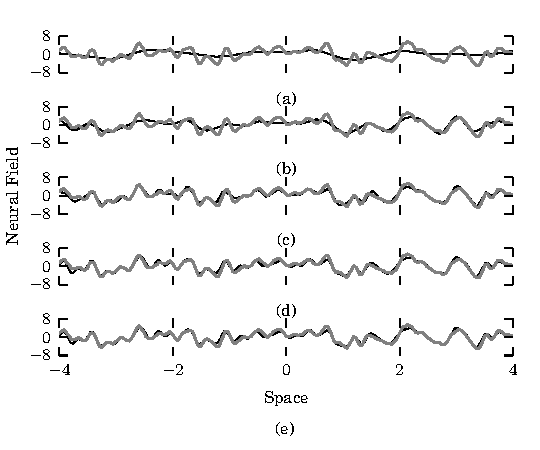
\includegraphics[scale=1]{./Graph/fig1.pdf}
	\caption{{\bf Multi-layer neural field model}. The inset figures show the shape of the
connectivity kernel components at each spatial resolution.}
	\label{fig:MultiLayerFieldModel}
\end{figure}
 
The multi-resolution structure has been described by numerous methods. For example, this idea of multi-resolution can be thought of a generalization of modeling the layers of the cortex separately, where the connectivity kernel, or neural foot-print, has varying widths \citep{Wilson1973}.

Typically, the experimentalist only has access the net field generated by the multi-resolution architecture of the cortex. Follow this, it is natural to ask how do we best describe the multi-resolution structure of the neural system. The solution to this problem was proposed by \citet{Breakspear2005} in using a wavelet decomposition. This paper is directed at developing a framework for patient-specific multi-resolution neural field models, forming a fundamental link between data and theory. 

\section{IDE Neural Field Model}
\singlespacing
\begin{table*}[!t]
\begin{tabular}{|l|l|l|}
	\hline
	\textbf{Symbol} & \textbf{Quantity} & \textbf{Units}\\
	\hline
	\multicolumn{3}{|c|}{\emph{Domain and indices}}\\
	\hline
	$\Omega$ & Spatial domain & n.a.\\
	$\mathbf{r}$ & Spatial location & [mm, mm]\\
	$t$ & Time & s\\
	\hline
	\multicolumn{3}{|c|}{\emph{Model}}\\
	\hline
    $y_t$ & Observation & mV\\
    $v(\mathbf{r},t)$ & Mean membrane potential & mV \\
	$f(v\left(\mathbf{r},t\right))$ & Firing rate function & spikes.s$^{-1}$\\
	$e_t(\mathbf{r})$ & Field disturbance, with covariance function $\eta(\mathbf r-\mathbf r')$ & mV\\
	$\boldsymbol\epsilon_t$ & Observation noise, with covariance matrix $\Sigma_\epsilon$ & mV\\
	$m(\mathbf{r}_n)$ & Observation kernel where $n$ is sensor index $n=1,..,n_y$ & n.a. \\
	$w(\mathbf{r})$ & Spatial connectivity kernel & n.a.\\
	$h(t)$ & Post-synaptic response kernel & mV\\
	$\tau$, $\xi$ & Membrane time constant \& time constant parameter & s, n.a.\\
	$\delta(t)$ & Dirac-delta function & n.a.\\
	\hline    
	\multicolumn{3}{|c|}{\emph{Multi-resolution Approximation}} \\
	\hline                                                   
	$\phi_{j,l}(r)$&Scaling function&n.a\\
	$\psi_{j,l}(r)$&Wavelet function&n.a\\  
	$\alpha_{j_0,l}, \beta_{j,l}$&Connectivity kernel approximation and detail coefficients&mV~spike$^{-1}$\\ 
	$x_{t,j_{0},l},\check{x}_{t,j,l}$&Field approximation and detail coefficients at a given time&mV~spike$^{-1}$\\ 
	$N_m(r)$&$m^{th}$ order B-spline function&n.a.\\
	$\varphi_m(r)$&$m^{th}$ order B-spline wavelet function&n.a.\\
	\hline
	\multicolumn{3}{|c|}{\emph{Reduced Model}} \\
	\hline
		$\boldsymbol\mu(r)$&Vector of $n_x$ field scaling and wavelet functions&n.a.\\
		$\boldsymbol\lambda(r)$&Vector of $n_{\boldsymbol\theta}$ connectivity kernel scaling and wavelet functions&n.a.\\
   	$\mathbf{x}_t$ & State vector at time $t$ composed of  $x_{t,j_{0},l}$ and $\check{x}_{t,j,l}$ & mV\\ 
		$\boldsymbol\theta$&Vector of connectivity kernel parameters composed of $\alpha_{j_0,l}$ and $\beta_{j,l}$& mV.spike$^{-1}$\\ 
		$\boldsymbol{\Lambda}_x$&Inner product of field basis functions&n.a.\\
		$\boldsymbol\Gamma, \boldsymbol\Lambda_{\boldsymbol{\theta}}$&Decomposition connectivity matrices&n.a.\\
   	$\mathbf{w}_t$ & State disturbance vector, with covariance $\Sigma_w$ & mV\\ 
    $\mathbf{A}(\boldsymbol{\theta})$& State transition matrix& n.a.\\
   	$\mathbf{C}$ & Observation matrix & n.a. \\
	\hline
	\multicolumn{3}{|c|}{\emph{Frequency Analysis}} \\
	\hline
	$\boldsymbol{\nu}$, $\boldsymbol{\nu}_c$ & spatial frequency and spatial cutoff frequency & cycles/mm \\
	$\sigma_{\nu}^2$ & variance of Fourier transformed Gaussian basis function & (cycles/mm)$^2$\\
	\hline
	\multicolumn{3}{|c|}{\emph{Estimation}} \\
	\hline
	$\hat{\mathbf{x}}_t^{f-}$, $\hat{\mathbf{x}}_t^f$ & Forward prior and posterior state estimates & mV\\
	$\hat{\mathbf{x}}_t^{b}$ & Backward posterior state estimates & mV\\
	$P^{f-}_t$, $P^f_t$  & Forward prior and posterior covariance matrices & mV$^2$\\
	$P^b_t$ & Backward posterior covariance matrices & mV$^2$\\
	$M_t$& Cross-covariance matrix & mV$^2$\\
	$\mathcal K_{t} $ & Filter gain & n.a.\\ 
	$\mathcal S_{t} $ & Smoother gain & n.a.\\ 
	$\boldsymbol\Xi_1, \boldsymbol\Xi_0$&Expected covariance and cross-covariance matrices& mV$^2$\\ 
	$\mathcal{Q}(\boldsymbol{\theta},\boldsymbol\theta')$&Lower bound on log-likelihood function&n.a.\\
	$\boldsymbol\nu_0$, $\boldsymbol\nu_1$&Lower bound coefficient matrices&n.a.\\ 
	$\boldsymbol\Upsilon$&Lower bound coefficient matrix&mV$^{-1}$.spike\\
	\hline
\end{tabular}
\caption{\textbf{Notation.} The first column of the table gives the symbols for all the notation used in the paper. The second column provides a brief description of the quantity, and the third column provides the SI units where relevant.}
\label{tab:Notation}
\end{table*}  
\doublespacing

The single layer homogeneous neural field model, in the most general form, is described by the equation
\begin{equation}
	\label{FullDoubleIntModel} \underbrace{v\left(\mathbf{r},t\right)}_{\text{field}} =
	\int_{-\infty}^t 
	\underbrace{h\left(t - t'\right)}_{\text{synapse}} \int_\Omega
	\parham{\theta}\underbrace{w\left(\mathbf{r},\mathbf{r}'\right)}_{\text{connectivity}} 
	\underbrace{f\left( v\left( \mathbf{r}',t' \right)\right)}_{\text{firing}}
	\, \mathrm{d}\mathbf{r}'\mathrm{d}t',
\end{equation}
where the post-synaptic membrane voltage at time $t$ of a population of neurons at position $\mathbf r$ within the spatial domain $\Omega$ is denoted by $v\left(\mathbf r,t\right)$. The function $h(t)$ describes the post-synaptic response kernel, $w\left(\mathbf{r},\mathbf{r}'\right)$ describes the connectivity kernel and $f(v(\mathbf{r},t))$ describes the relationship between the mean membrane potential and the mean firing rate. The parameter $\theta$ can be thought of the synaptic efficiency or coupling strength, where $\theta>0$ and $\theta<0$ describes excitation and inhibition, respectively. There are various forms of $h(t)$ that have been proposed in the literature, with different levels of complexity. These are shown in Fig.~\ref{fig:Modelcomponents}. Similarly, both the connectivity kernel and the activity function (firing rate) can take various forms. These are also shown in Fig.~\ref{fig:Modelcomponents}. The form of $w(\mathbf{r},\mathbf{r}')$ typically describes an Laplacian (exponential) or Gaussian decay in connectivity strength from any point in the field. By assuming the form of $h(t)$ is the same across layers (scales) the Amari style neural field model is formed, incorporating a multilayer structure into the connectivity kernel. In this way, the connectivity kernel typically takes the form of a Mexican hat (Gaussian shape within layer connectivity) or Wizard hat (Laplacian shape within layer) as depicted in Fig.~\ref{fig:Modelcomponents}.

The stochastic IDE form of the Amari neural field formulation~\cite{Amari1977} is given by (see~\cite{Freestone2011} for a full derivation)
\begin{equation}\label{eq:DiscreteTimeModel}
	v_{t+1}\left(\mathbf{r}\right) = 
	\xi v_t\left(\mathbf{r}\right) + 
	T_s \int_\Omega { 
	    w\left(\mathbf{r},\mathbf{r'}\right)
	    f\left(v_t\left(\mathbf{r}'\right)\right) 
	\, \mathrm{d}\mathbf{r}'} 
	+ e_t\left(\mathbf{r}\right), 
\end{equation}
where in this first-order (in time) form of the model the membrane dynamics are included through the parameter $\xi=1-T_s/\tau$, $\tau$ is the membrane time constant and $T_s$ is the sampling time step. 
% The connectivity strength between neural populations at a distance $\mid\mathbf{r}-\mathbf{r'}\mid$ is described by the connectivity kernel $w\left(\mathbf{r}-\mathbf{r}'\right)$. The connectivity kernel is taken as a ``Mexican hat'' function, which describes local excitation and lateral inhibition \cite{Amari1977,Atay2005}. The components of the model are shown in Fig.~\ref{fig:Modelcomponents}
\begin{figure}[!t]
\centering
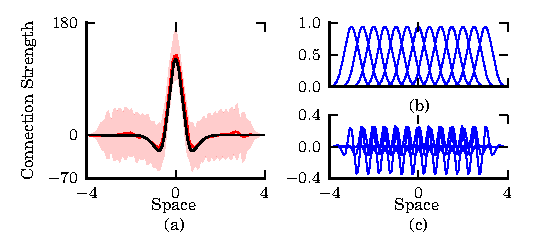
\includegraphics[scale=1]{./Graph/fig2.pdf}
\caption{ {\bf The IDE neural field model components}. (\textbf{A}) The Mexican hat (dotted line) and Wizard hat (solid line) connectivity kernels. (\textbf{B}) First order (dotted line) and second order (solid line) synaptic kernels. (\textbf{C}) A representative of the activation function.}
\label{fig:Modelcomponents}
\end{figure}
The term $e_t(\mathbf r)$ is a zero mean Gaussian disturbance, spatially colored but temporally white, with covariance function 
\begin{equation}
cov\left(e_{t}\left(\mathbf{r}\right),e_{t+t'}\left(\mathbf{r'}\right)\right)=\sigma_d\eta(\mathbf{r}-\mathbf{r'})\delta(t-t'),
\label{eq:FieldDisturbance}
\end{equation}
where \parham{$\eta(\mathbf{r}-\mathbf{r'})$ is a spatially homogeneous covariance function, $\sigma_d$ is disturbance variance} and $\delta(\cdot)$ is the Dirac-delta function. %$ = \varsigma v_t(\mathbf{r})$ \cite{VanRotterdam1982,Murphy2009}.

The observation equation describing the intracranial electrophysiological recordings is given by
\begin{equation}\label{eq:ObservationEquation}
	y_t(\mathbf{r}_{n_y}) = \int_{\Omega} { m\left(\mathbf{r}_{n_y}-\mathbf{r}'\right) v_t\left(\mathbf{r}'\right) \, \mathrm{d}\mathbf{r}'} + \epsilon_t(\mathbf{r}_{n_y}), 
\end{equation}
where $m\left(\mathbf{r}_{n_y}-\mathbf{r}'\right)$ is the observation kernel at location $\mathbf{r}_{n_y}$ and  $\boldsymbol{\epsilon}_{t}\sim \mathcal{N}\left(\mathbf{0},\mathbf{\Sigma}_{\epsilon}\right)$  is an i.i.d. Gaussian white noise process and the covariance matrix $\mathbf{\Sigma}_{\epsilon}=\sigma^2_{\epsilon}\mathbf I_{n_y}$, where $\mathbf I$ denotes the identity matrix. The observation kernel models the pickup range of the electrical fields of the brain. The lead field parameters are not included in the observation equation as the intracranial recordings are considered here. 

\section{MRA of the IDE in State-Space}
The purpose of forming the multi-resolution approximation (MRA) of the integro-difference equation (IDE) is to form a multi-resolution finite-dimensional state-space model that best captures the spatiotemporal characteristics of the neural field. Given such a model, it is then possible to perform state and parameter estimation in an efficient and robust manner, thus allowing for subject-specific models. The goal of this section is to demonstrate how to formulate a state-space model in a canonical form such that standard algorithms may be applied to estimate the multi-resolution connectivity structure.   
% form a parameterized equation for coefficients of the field basis functions $\mathbf{x}_t$, which becomes the state vector.

The multi-resolution approximation \citep{Mallat1989a} of the neural IDE (MRAIDE) is obtained by decomposing both the field, $v_t(\cdot)$, and the connectivity kernel, $w(\cdot)$, (assuming square-integrable functions) using translations and dilations of a scaling function $\phi(\mathbf{r})$ and a mother wavelet $\psi(\mathbf{r})$. Considering a  one-dimensional field, the static connectivity kernel is decomposed as,
\begin{equation}
 w\left(r\right)=\sum_{l\in \mathbb{Z}}\alpha_{j_0,l} \underbrace{\phi_{j_0,l}\left(r\right)}_{\text{scaling functions}} + \sum_{j\geq j_0}^{\infty} \sum_{l \in \mathbb{Z}}\beta_{j,l} \underbrace{\psi_{j,l}\left(r\right)}_{\text{wavelets}}, 
\label{eq:KernelExpansion}
\end{equation}
where $\alpha_{j_0,l}$ are the approximation coefficients at the lowest scale $j_0$, and $\beta_{j,l}$ are the detail coefficients at different scales $j$, with
\begin{align}
\phi_{j,l}\left(r\right) =& 2^{\frac{j}{2}}\phi\left(2^j r-l\right) \label{eq:generalscalingfinction}\\	
\psi_{j,l}\left(r\right) =& 2^{\frac{j}{2}}\psi\left(2^j r-l\right).  \label{eq:generalwaveletfinction}
\end{align}
The parameters $j$ and $l$ control the scale (dilation) and translation (spatial shift), respectively. The number of spatial shifts, $l$, is dependent on the scale, $j$, and can be chosen such that the basis functions cover the spatial domain of interest. For example, at scales corresponding to higher spatial frequencies a greater number of wavelets, and thus spatial shifts are required to adequately sample the spatial characteristics of the field. The number of scales depends on the spectral characteristics of the field, where higher spatial frequencies require a more scales. Spatial frequency analysis will be described later in Section~\ref{sec:freq_anal} in greater detail. Scaling functions retain the lowest frequency components, due to their low-pass properties, while the wavelet functions extract successively higher frequency components due to their band-pass characteristics. 

% At each spatial scale indexed by $j$ (level of decomposition), the neural field can be written as
% \begin{equation}
% 	v_{j,t}\left(\mathbf{r}\right) = \begin{cases}
% 	\sum_{l \in \mathbb{Z}}x_{j,l}(t) \underbrace{\phi_{j,l}\left(\mathbf{r}\right)}_{\text{scaling function}} + \check{x}_{t,j,l}\underbrace{\psi_{j,l}\left(\mathbf{r}\right)}_{\text{mother wavelet}} & \text{if $j=0$},\\
% 	\sum_{l \in \mathbb{Z}}\check{x}_{t,j,l}\psi_{j,l}\left(\mathbf{r}\right) & \text{otherwise}
% \end{cases}
% \end{equation}
The dynamic neural field is decomposed using
\begin{equation}
 v_t\left(r\right)=\sum_{l \in \mathbb{Z}}x_{t,j_{0},l} \underbrace{\phi_{j_0,l}\left(r\right)}_{\text{scaling functions}} + \sum_{j\geq j_0}^{\infty} \sum_{l \in \mathbb{Z}} \check{x}_{t,j,l} \underbrace{\psi_{j,l}\left(r\right)}_{\text{wavelets}},
\label{eq:FieldExpansion}
\end{equation}
where $x_{t,j_{0},l}$ and $\check{x}_{t,j,l} $ are the dynamic coefficients of the expansion, constituting the state vector at time $t$. The decomposition enables a separation of the static spatial characteristics, which are considered static functions, that are weighted by dynamic coefficients.

Eqs.~\eqref{eq:KernelExpansion} and \eqref{eq:FieldExpansion} are infinite series expansions and must be truncated to some level $j,$ in order to solve the estimation problem. In other words, the neural field must be band-limited up to a given spatial frequency. 

Now we will simplify the notation by defining vectors that contain all the translations of the wavelets and scaling functions 
\begin{align}      
	\boldsymbol\phi_{j_0}(r) \triangleq&\left\lbrace{\phi_{j_0,l}(r)}:l \in \mathbb{Z} \right\rbrace \\
	\boldsymbol\psi_{j}(r) \triangleq& \left\lbrace{\psi_{j,l}(r)}:l \in \mathbb{Z} \right\rbrace\\
	\boldsymbol\alpha_{j_0} \triangleq& \left\lbrace\alpha_{j_0, l}:l \in \mathbb{Z} \right\rbrace \\
	\boldsymbol\beta_{j} \triangleq& \left\lbrace\beta_{j, l}:l \in \mathbb{Z} \right\rbrace \\
	\mathbf{x}_{t,j_0} \triangleq& \left\lbrace{x}_{t,j_{0},l}:l \in \mathbb{Z} \right\rbrace \\
	\check{\mathbf{x}}_{t,j} \triangleq& \left\lbrace{\check{x}}_{t,j,l}:l \in \mathbb{Z} \right\rbrace.
\end{align}
Following this we can define the vectors 
\begin{align}
\boldsymbol\theta^\top \triangleq& [\begin{array}{ccccc} \boldsymbol\alpha_{j_0}^\top & \boldsymbol\beta_{j_0}^\top & \boldsymbol\beta_{j_0+1}^\top & \cdots & \boldsymbol\beta_{j}^\top \end{array}] 
\label{KernelWeights} \\
\mathbf{x}_{t}^\top \triangleq& [\begin{array}{ccccc}\mathbf{x}_{t,j_{0}}^\top &  \check{\mathbf{x}}_{t,j_{0}}^\top & \check{\mathbf{x}}_{t,j_{0}+1}^\top & \cdots & \check{\mathbf{x}}_{t,j}^\top\end{array}]
\label{FieldWeights} \\
\label{KernelBasisVector}
\boldsymbol\lambda^\top(r) \triangleq& \left[
\begin{array}{ccccc} \boldsymbol\phi_{j_0}^\top(r) &
\boldsymbol\psi_{j_0}^\top(r) & 
\boldsymbol\psi_{j_0+1}^\top(r) &
\cdots &
\boldsymbol\psi_{j}^\top(r)\end{array}\right] \\
\label{FieldBasisVector}
\boldsymbol\mu^\top (r) \triangleq& \left[
\begin{array}{ccccc}\boldsymbol\phi_{j_0}^\top(r) &
\boldsymbol\psi_{j_0}^\top(r) & 
\boldsymbol\psi_{j_0+1}^\top(r) &
\cdots &
\boldsymbol\psi_{j}^\top(r)\end{array}\right],
\end{align}
which allow us to write the neural field and connectivity kernel decomposition in the compact form of
\begin{align}
	w\left(r\right) &\approx \boldsymbol\theta^\top\boldsymbol\lambda\left(r\right) 
	\label{eq:KernelFiniteExpansion} \\
	v_t\left(r\right) &\approx \boldsymbol\mu^\top\left(r\right)\mathbf{x}_t.
	\label{eq:FieldFiniteExpansion}
\end{align}
% where the unknown parameter and state vectors, $\boldsymbol\theta \in \mathbb{R}^{n_{\theta}}$ and $\mathbf{x}_t \in \mathbb{R}^{n_x}$, \dean{($\boldsymbol\theta \in \mathbb{R}^{n_{\theta}\times (J+2)}$ and $\mathbf{x}_t \in \mathbb{R}^{n_x \times (J+2)}$)} are defined as 
% \begin{align}
% \boldsymbol\theta^\top \triangleq& [\begin{array}{ccccc} \boldsymbol\alpha_{j_0}^\top & \boldsymbol\beta_{j_0}^\top & \boldsymbol\beta_{j_0+1}^\top & \cdots & \boldsymbol\beta_{J}^\top \end{array}] 
% \label{KernelWeights} \\
% \mathbf{x}_{t}^\top \triangleq& [\begin{array}{ccccc}\mathbf{x}_{t,j_{0}}^\top &  \check{\mathbf{x}}_{t,j_{0}}^\top & \check{\mathbf{x}}_{t,j_{0}+1}^\top & \cdots & \check{\mathbf{x}}_{t,J}^\top\end{array}].
% \label{FieldWeights}
% \end{align}
% The kernel and field approximation coefficient vectors, $\boldsymbol \alpha_{j_0}$ and $\mathbf{x}_{t,j_{0}}$, contain all the coefficients $\left\lbrace\alpha_{j_0, \mathbf{l}}:\mathbf{l} \in \mathbb{Z}^n \right\rbrace $ and $\left\lbrace x_{t,j_0, \mathbf{l}}: \mathbf{l} \in \mathbb{Z}^n\right\rbrace$, respectively. Similarly, the kernel and the field detail coefficient vectors, $\boldsymbol\beta_{j}$ and $\check{\mathbf{x}}_{t,j}$, contain all the coefficients $\left\lbrace \beta_{j,\mathbf{l}} :\mathbf{l} \in \mathbb{Z}^n\right\rbrace$ and $\left\lbrace  \check x_{t,j,\mathbf{l}}:\mathbf{l} \in \mathbb{Z}^n\right\rbrace$, respectively.
% 
% The vectors of the kernel and the field scaling and wavelet functions, $\boldsymbol\lambda$ and $\boldsymbol\mu$, respectively, are defined by
% \begin{align}
%     \label{KernelBasisVector}
%     \boldsymbol\lambda^\top(\mathbf{r}) \triangleq& \left[
%     \begin{array}{ccccc} \boldsymbol\phi_{j_0}^\top(\mathbf{r}) &
%     \boldsymbol\psi_{j_0}^\top(\mathbf{r}) & 
%     \boldsymbol\psi_{j_0+1}^\top(\mathbf{r}) &
%     \cdots &
%     \boldsymbol\psi_{J}^\top(\mathbf{r})\end{array}\right] \\
%     \label{FieldBasisVector}
%     \boldsymbol\mu^\top (\mathbf{r}) \triangleq& \left[
%     \begin{array}{ccccc}\boldsymbol\phi_{j_0}^\top(\mathbf{r}) &
%     \boldsymbol\psi_{j_0}^\top(\mathbf{r}) & 
%     \boldsymbol\psi_{j_0+1}^\top(\mathbf{r}) &
%     \cdots &
%     \boldsymbol\psi_{J}^\top(\mathbf{r})\end{array}\right]
% \end{align}
% 
% The vectors in  (\ref{KernelBasisVector}) and (\ref{FieldBasisVector}) are constructed in the same manner as the vectors in  (\ref{KernelWeights}) and (\ref{FieldWeights}).  
Now we have the compact form of the decomposition we can substitute this into the neural field Eq.~\eqref{eq:DiscreteTimeModel} giving
\begin{equation}\label{eq:ApproxDiscreteTimeModel}
	\boldsymbol\mu^\top\left(r\right)\mathbf{x}_{t+1} = 
	\xi \boldsymbol\mu^\top\left(r\right)\mathbf{x}_t + 
	T_s \int_\Omega { 
	    \boldsymbol\theta^\top\boldsymbol\lambda\left(r-r'\right)
	    f\left(\boldsymbol\mu^\top\left(r'\right)\mathbf{x}_t\right) 
	\, \mathrm{d}r'}  
	+ e_t\left(r\right).
\end{equation}
The aim of the next part of the derivation is to isolate the state vector on the left hand side of the equation. To do this we first multiply both sides of Eq.~\eqref{eq:ApproxDiscreteTimeModel} by $\boldsymbol\mu\left(r\right)$ and integrate over space giving 
\begin{align}\label{eq:ApproxDiscreteTimeModel2}
	\int_{\Omega} \boldsymbol\mu\left(r\right)\boldsymbol\mu^\top\left(r\right) \mathrm{d}r \mathbf{x}_{t+1} &= 
	\xi \int_{\Omega}\boldsymbol\mu\left(r\right)\boldsymbol\mu^\top\left(r\right) \mathrm{d}r \mathbf{x}_t + 
	T_s \int_{\Omega}\boldsymbol\mu\left(r\right)\int_\Omega { 
	    \boldsymbol\theta^\top\boldsymbol\lambda\left(r-r'\right)
	    f\left(\boldsymbol\mu^\top\left(r'\right)\mathbf{x}_t\right) 
	\, \mathrm{d}r'\mathrm{d}r}  \nonumber\\
	&+ \int_{\Omega}\boldsymbol\mu\left(r\right)e_t\left(r\right)\mathrm{d}r.
\end{align}
To isolate the state vector, we now define the matrix 
\begin{equation}
	\label{eq:Lambdax}
	 \mathbf{\Lambda}_{x} \triangleq \int_{\Omega}\boldsymbol{\mu}\left(r\right)\boldsymbol{\mu}^\top\left(r\right) \mathrm{d}r,
\end{equation}
and substitute into Eq.~\eqref{eq:ApproxDiscreteTimeModel2} giving
\begin{equation}\label{eq:ApproxDiscreteTimeModel3}
	\mathbf{\Lambda}_{x} \mathbf{x}_{t+1} = 
	\xi \mathbf{\Lambda}_{x} \mathbf{x}_t + 
	T_s \int_{\Omega}\boldsymbol\mu\left(r\right)\int_\Omega { 
	    \boldsymbol\theta^\top\boldsymbol\lambda\left(r-r'\right)
	    f\left(\boldsymbol\mu^\top\left(r'\right)\mathbf{x}_t\right) 
	\, \mathrm{d}r'\mathrm{d}r}  
	+ \int_{\Omega}\boldsymbol{\mu}\left(r\right) e_t\left(r\right) \mathrm{d}r.
\end{equation}
Cross-multiplying by $\mathbf{\Lambda}_{x}^{-1}$ gives the state transition equation
\begin{equation}\label{eq:ApproxDiscreteTimeModel4}
	\mathbf{x}_{t+1} = 
	\xi \mathbf{x}_t + 
	T_s \mathbf{\Lambda}_{x}^{-1} \int_{\Omega}\boldsymbol\mu\left(r\right)\int_\Omega { 
	    \boldsymbol\theta^\top\boldsymbol\lambda\left(r-r'\right)
	    f\left(\boldsymbol\mu^\top\left(r'\right)\mathbf{x}_t\right) 
	\, \mathrm{d}r'\mathrm{d}r}  
	+ \mathbf{\Lambda}_{x}^{-1}\int_{\Omega}\boldsymbol{\mu}\left(r\right) e_t\left(r\right) \mathrm{d}r.
\end{equation}
A very nice property of the MRAIDE framework is the disturbance term becomes a vector valued, zero-mean normally distributed, white noise process 
\begin{equation}\label{eq:Disturbance}
\mathbf w_t= \mathbf{\Lambda}_{x}^{-1}\int_{\Omega}\boldsymbol\mu \left(r\right)e_t\left(r\right)\,\mathrm{d}r,
\end{equation}
with covariance (see \citet{Freestone2011} for proof)
\begin{equation}\label{eq:CovMatrix}
\boldsymbol\Sigma_w =\mathbf{\Lambda}_{x}^{-1}\iint\limits_{\boldsymbol\Omega}\boldsymbol\mu\left(r\right) \eta\left(r-r'\right)\boldsymbol\mu^{\top}\left(r'\right)\,\mathrm{d}r'\mathrm{d}r\mathbf{\Lambda}_{x}^{-\top}.
\end{equation} 

The state-transition equation can be simplified if the chosen family of scaling and wavelet functions are isotropic where
\begin{equation}
	\boldsymbol{\lambda}_{i}(r-r') = \boldsymbol{\lambda}(2\mathbf{c}_{i}+r'-r), 
\end{equation}
where $c_i$ is the centre of the $i^{th}$ basis function of the kernel decomposition. Following this, we can switch the order of operations with the inner product and convolution in Eq.~\eqref{eq:ApproxDiscreteTimeModel4}. With this switch the convolution is now between the scaling functions and wavelets for the field and the scaling functions and wavelets for the connectivity kernel. This convolution can be calculated analytically when using B-spline scaling and wavelet functions and can be predefined, since these are static functions. This has major computation advantages when solving the estimation problem. %\parham{Although this switch holds theoretically it should be noted that it will introduce numerical error, specially close to the edges, due to the finite extent of the field. } 
The predefined convolution can be written as
\begin{equation}\label{eq:Gammaij}
	\left[\Gamma(r')\right]_{:i} = T_s \mathbf{\Lambda}_{x}^{-1}\int_{\Omega} \boldsymbol\mu\left(r\right)\boldsymbol\lambda\left(2c_{i} + r'-r\right) \,\mathrm{d}r,
\end{equation} 
 where $\left[\Gamma(r')\right]_{:i}$ denotes the $i^{th}$ column of  $\left[\Gamma(r')\right]$ giving
\begin{equation}
	\mathbf{x}_{t+1} = 
	\xi \mathbf{x}_t + 
	\int_{\Omega} \Gamma\left(r'\right)f\left(\boldsymbol\mu^\top\left(r'\right) \mathbf{x}_t\right) 
	\, \mathrm{d}r' \boldsymbol\theta
	+ \mathbf w_t.
\end{equation}
% Substituting Eq.~\eqref{eq:KernelFiniteExpansion} and Eq.~\eqref{eq:FieldFiniteExpansion} in Eq.~\eqref{eq:DiscreteTimeModel}, pre-multiplying by $\boldsymbol\mu\left(r\right)$, and integrating over the space gives
% \begin{align}\label{eq:DecomposedModel2} 
% 	&\mathbf{\Lambda}_{x} \mathbf{x}_{t+1} = 
% 	\xi\mathbf{\Lambda}_{x} \mathbf{x}_t +T_s \varsigma \mathbf{\Lambda}_{\theta}\mathbf{x}_t +\int_{\Omega}\boldsymbol\mu\left(r\right)e_t\left(r\right)dr.
% \end{align}
% Cross-multiplying by $\mathbf{\Lambda}_{x}^{-1}$ gives the state transition equation
% \begin{align}\label{eq:StateEquation}
%  \mathbf x_{t+1} &=\mathbf A(\boldsymbol \theta) \mathbf x_t+ \mathbf w_t\\
% \label{eq:A_theta}
%  \mathbf A(\boldsymbol \theta) &= T_s\varsigma\mathbf{\Lambda}_{x}^{-1}\mathbf{\Lambda}_{\theta}+\xi\mathbf I.
% \end{align}
% The disturbance becomes 
% \begin{equation}\label{eq:Disturbance}
% \mathbf w_t= \mathbf{\Lambda}_{x}^{-1}\int_{\Omega}\boldsymbol\mu \left(r\right)e_t\left(r\right)dr,
% \end{equation}
% which is a vector valued, zero-mean normally distributed, white noise process with covariance (see \cite{Freestone2011} for proof)
% \begin{equation}\label{eq:CovMatrix}
% \boldsymbol\Sigma_w =\mathbf{\Lambda}_{x}^{-1}\iint\limits_{\boldsymbol\Omega}\boldsymbol\mu\left(r\right) \eta\left(r-r'\right)\boldsymbol\mu^{\top}\left(r'\right)dr'dr\mathbf{\Lambda}_{x}^{-\top}.
% \end{equation}
The observation equation of the state-space model is found by substituting decomposition \eqref{eq:FieldFiniteExpansion}
 into Eq.~\eqref{eq:ObservationEquation} giving
\begin{equation}\label{eq:ReducedObservationEquation} 
	\mathbf{y}_t = \mathbf{C}\mathbf{x}_t + \boldsymbol{\epsilon}_t,
\end{equation}
where each element of the observation matrix, $\mathbf{C}$, is given by
\begin{equation}\label{eq:Observationmatrix}
	\mathbf{C}_{ik} \triangleq \int_{\Omega}m(r_i -r')\boldsymbol{\mu}_k(r') \, \mathrm{d}r'.
\end{equation}
\section{B-Spline MRAIDE in State-Space }
\subsection{A Brief Introduction to B-Spline Wavelets}
B-spline functions are one of the most basic elements for wavelet construction. These functions are composed of piecewise polynomials combined smoothly at some breaking points (knots), which are equally spaced in the case of cardinal B-splines. The degree of smoothness is determined by the order of splines \citep{Goswami1999}, where the higher the order the smoother the resulting B-spline becomes (see Fig.~\ref{fig:Figure0}).
\begin{figure}[!t]
\centering
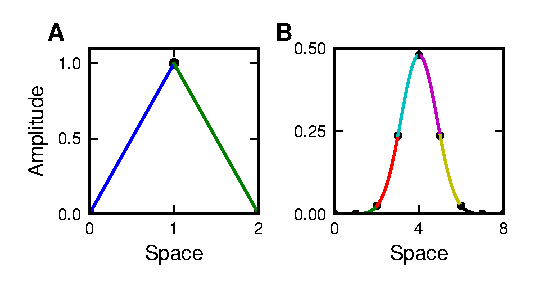
\includegraphics{./Graph/fig3.pdf}
% 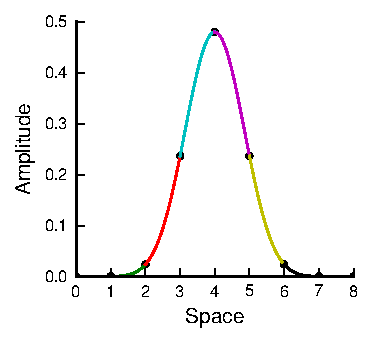
\includegraphics{./Graph/Figure0b.pdf}
\caption{{\bf Examples of cardinal B-spline functions}. Piecewise polynomial functions (colored lines) are joined at the break points (black dots). (\textbf{A}) B-spline function of order 2 (linear B-spline). (\textbf{B}) B-spline function of order 8.}
\label{fig:Figure0}
\end{figure}
 
B-spline wavelet and scaling functions were formulated independently by \citet{Chui1992b}, \citet{Chui1992} and \citet{Unser1993}.  The scaling functions are $m^{th}$ order B-splines and the compact support wavelet functions are a linear combination of scaling functions. B-spline wavelet and scaling functions approach optimal time/frequency localization as the order of the spline increases. In fact, for the cubic B-spline scaling and wavelet functions it is already close to the optimal limit for Gaussian functions \citep{Unser1999}. 
%and they have a better approximation rate than other wavelets with the same number of vanishing moments 

B-spline wavelet and scaling functions are particularly suited in this framework due to the property of being able to analytically define the convolution and inner product to form MRAIDE components. The following summarizes some important characteristics of B-splines relevant to the proposed modeling framework. 

The $m^{th}$  order cardinal B-spline function is defined by the recurrence relation \citep{Chui1992} 
\begin{equation}
N_{m}\left(r\right) = \left(N_{m-1}\ast N_{1}\right)\left(r\right) = \int_0^{1} N_{m-1}\left( r-r'\right)\,\mathrm{d}r',
\label{SplineConvolutionIntegral}
\end{equation}
where $m>1$, $\ast$ denotes convolution, and $N_1\left(r\right)$ is the characteristic function of the unit interval $\left[ 0,1\right)$, also known as indicator function, i.e.
\begin{equation}
N_{1}\left(r\right)=
\begin{cases}
1 & \text{if $ 0\le r<1$}, \\
0 & \mathrm{elsewhere}.
\end{cases}
\end{equation}
Following this, a B-spline of any order, $N_m(r)$, can be computed using the recursive expression defined by \citet{DeBoor2001}
\begin{equation}\label{eq:MRA-DoBoorFormula}
 N_{m}\left(r\right)=\frac{r}{m-1}N_{m-1}\left(r\right)+\frac{m-r}{m-1}N_{m-1}\left(r-1\right) \quad m>1.
 \end{equation}
The most commonly used form of splines is the cubic spline $\left(m=4\right)$, comprised of third degree polynomials added together at the joining points, with an explicit expression given by
\begin{align}
3!N_{4}\left(r\right)=
\begin{cases}
r^3 & \text{if $ 0\le r\le1$}, \\
4-12r+12r^2-3r^3 & \text{if $1\le r\le2$}, \\
-44+60r-24r^2+3r^3 & \text{if $2\le r\le3$}, \\
64-48r+12r^2-r^3 & \text{if $3\le r\le4$}, \\
0 & \mathrm{elsewhere}.
\end{cases}
\end{align}
One important feature of the B-spline functions is the \emph{partition of unity} property, meaning that the unity can be expressed as a linear sum of B-splines, i.e
\begin{equation}
	\sum_{l}N_m(r+l)\equiv1.
	\end{equation}
This is important as the underlying field can be reconstructed when it is saturated without introducing numerical errors which is not the case for example when Gaussian basis functions are used.
	
The convolution and inner product of B-spline functions are required in order to formulate the multi-resolution framework described in the previous section (construction of $\boldsymbol\Lambda_{x}$ and $\boldsymbol\Gamma$). To show how the convolution of two B-splines is calculated, Eq.~\eqref{SplineConvolutionIntegral} can be rewritten as $(m-1)$ convolutions of the indicator function with itself
\begin{equation}\label{eq:N1convolutions}
 N_{m}\left(r\right)=\underbrace{\left(N_{1}\ast N_{1}\ast \cdots \ast N_{1}\right)}_{m-1\quad \text{convolutions}}\left(r\right).
\end{equation}
Using the associativity property of convolution, we have
\setlength{\arraycolsep}{0.0em}
\begin{align}\label{eq:BsplineConvolution}
N_{m}\left( r\right) \ast N_{m'}\left(r\right)&=\underbrace{\overbrace{\left(N_{1} \ast \cdots \ast N_{1}\right)}^{m-1 \quad \text{convolutions}}\left(r\right) \ast \overbrace{\left(N_{1} \ast \cdots \ast N_{1}\right)}^{m'-1\quad \text{convolutions}}}_{m+m'-1 \quad \text{convolutions}}\left(r\right)\nonumber\\
&=N_{m+m'}\left(r\right).
\end{align}
A direct consequence of Eq.~\eqref{eq:BsplineConvolution} is the inner product between two B-splines is another translated B-spline such that
\begin{align}
 \left\langle N_{m}\left(r-l_{1}\right), N_{m'}\left(r-l_{2}\right)\right\rangle=&N_{m+m'}\left(m+l_{1}-l_{2}\right)\nonumber \\
=&N_{m+m'}\left(m'+l_{2}-l_{1}\right),
\label{eq:BsplineInnerProduct}
\end{align}
where $\left\langle \cdot,\cdot\right\rangle $ denotes the inner product. This holds as the support of $N_m\left(r\right)$ is $\left[ 0,m\right]$ and  is symmetric with respect to $r=\frac{m}{2}$, i.e. $ N_{m}\left(\frac{m}{2}+r\right)=N_{m}\left(\frac{m}{2}-r\right)$ (see \ref{ap:InnerProductOfBsplines} for explicit derivation). The values of $N_{m+m'}$ in Eq.~\eqref{eq:BsplineInnerProduct} can be easily determined recursively by evaluating Eq.~\eqref{eq:MRA-DoBoorFormula} at integer points, i.e.
 \begin{equation}\label{eq:MRA-recursiveBsplineatintegerpoints}
 \begin{cases}
 N_2(k)=\delta(k-1)\quad k\in \mathbb{Z}, \\
 N_{m}\left(k\right)=\frac{k}{m-1}N_{m-1}\left(k\right)+\frac{m-k}{m-1}N_{m-1}\left(k-1\right) \quad k=1,2,\dots,m-1.
  \end{cases}
 \end{equation}
Note $N_{m}\left(k\right)=0$ for $k\le0$ or $k\ge m$. 

The multi-resolution approximation using B-spline functions is completed by defining a two-scale relation pair, which relates the scaling functions and the wavelets at a given scale with the scaling function at the next higher scale. For cardinal B-spline scaling and wavelet functions of order $m$ the two-scale relation pair takes the form of
\begin{align}
 N_{m}\left(r\right)&=\sum_{n=0}^{m} \left[\mathbf p\right]_n N_{m}\left(2r-n\right) \label{eq:MRA-TwoScalepair1} \\
  \varphi_{m}\left(r\right) &= \sum_{n=0}^{3m-2}  \left[\mathbf q\right]_n N_{m}\left(2r-n\right)\label{eq:MRA-TwoScalepair2},
 \end{align}
where 
 \begin{align}
\left[\mathbf p\right]_n&=2^{-m+1} \binom{m}{n} \quad \text{ $0\le n\le m$} \label{eq:MRA-TwoScalepair1coefs}\\
\left[\mathbf q\right]_n&= \left(-1\right)^n{2^{-m+1}}\sum_{l=0}^{m} \binom{m}{l} N_{2m}\left(n-l+1\right), \,  \text{ $0\le n\le 3m-2$}\label{eq:MRA-TwoScalepair2coefs}
 \end{align}
and $\left[\cdot\right]_n$ denotes the $n^{th}$ element of the vector coefficients \citep{Chui1992}.

Fig.~\ref{fig:MRA-Figure1} shows the cubic B-spline scaling function and its associated wavelet function with dilation and translation parameters set to zero. Note in general the supports of B-spline scaling and wavelet functions are given by 
\begin{align}
	\mathrm{supp}(N_{m;j,l})&=\left[\frac{l}{2^j},\frac{m+l}{2^j}\right] \label{eq:ScalingSupport}\\  
  \mathrm{supp}(\varphi_{m;j,l})&=\left[\frac{l}{2^j},\frac{2m-1+l}{2^j}\right],\label{eq:WaveletSupport}
	\end{align}    
where subscripts $j$ and $l$ in Eqs.~\eqref{eq:ScalingSupport} and \eqref{eq:WaveletSupport} are introduced to $N_{m}(r)$ and $\varphi_{m}(r)$ to indicate the scale and translation parameters as defined in Eqs~\eqref{eq:generalscalingfinction} and \eqref{eq:generalwaveletfinction}.
\begin{figure}[!t]
\centering
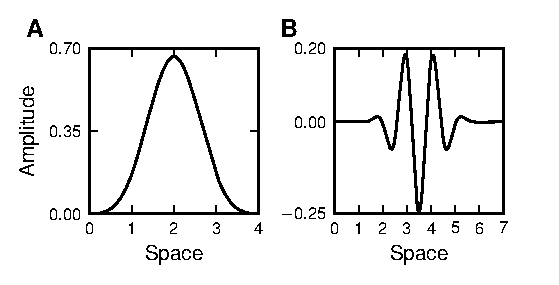
\includegraphics{./Graph/fig4.pdf}
% 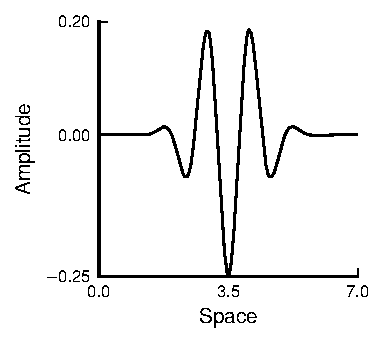
\includegraphics{./Graph/Figure1b.pdf}
\caption{{\bf Examples of B-spline scaling and wavelet functions}. (\textbf{A}) The cubic B-spline scaling function. (\textbf{B}) The corresponding wavelet function.}
\label{fig:MRA-Figure1}
\end{figure}
 
By exploiting Eq.~\eqref{eq:BsplineConvolution} and Eq.~\eqref{eq:BsplineInnerProduct}, the integrals in Eq.~\eqref{eq:Lambdax} and Eq.~\eqref{eq:Gammaij} can be computed analytically. In constructing $\boldsymbol\Lambda_{x}$, it is important to note that B-spline scaling and wavelet functions possess the following orthogonality properties \citep{Unser1993}: 
\begin{equation}
  \left\langle \varphi_{m;j_1,l_1}(r),\varphi_{m;j_2,l_2}(r)\right\rangle =0  \quad \mathrm{for} \quad j_1\neq j_2
 \label{eq:MRA-PsiPsiOrthogonality} 
 \end{equation}
 \begin{equation}
  \left\langle N_{m;j_1,l_1}(r),\varphi_{m;j_2,l_2}(r)\right\rangle =0  \quad \mathrm{for} \quad j_1\leq j_2.
 \label{eq:MRA-PhiPsiOrthogonality}
 \end{equation}
Note from Eq.~\eqref{eq:MRA-PsiPsiOrthogonality} B-spline wavelets are semi-orthogonal as they are not orthogonal with respect to translation on a given scale.

In order to analytically calculate elements of $\boldsymbol\Lambda_{x}$ and $\boldsymbol\Gamma$, the scaling and wavelet basis functions must be expanded in terms of $N_m$ at the appropriate scale using the two-scale relation pair defined in Eqs.~(\eqref{eq:MRA-TwoScalepair1}-\eqref{eq:MRA-TwoScalepair2coefs}). For scaling functions this can be done  by using Eq.~\eqref{eq:MRA-TwoScalepair1} recursively, giving
\begin{align}\label{eq:MRA-ConvertingFormulaForscalingFunctions}
 &N_m(r)=\nonumber \\
&\sum_{n_1,n_2, \dots n_j=0}^{m}\left[\mathbf p\right]_{n_1} \left[\mathbf p\right]_{n_2}\dots \left[\mathbf p\right]_{n_j}N_m(2^jr-l_{n_1,n_2, \dots, n_j}),
\end{align}
where 
\begin{align}
 l_{n_1,n_2, \dots, n_j}=2^{j-1}n_1+2^{j-2}n_2+ \dots +2^{0}n_j.
\end{align}
The relation \eqref{eq:MRA-ConvertingFormulaForscalingFunctions} can be also proven by induction (see \ref{ap:Induction}). A similar method can be used for wavelet functions noting that they must be written first in terms of scaling functions using Eq.~\eqref{eq:MRA-TwoScalepair2}. Examples of such expansions are given in Fig.~\ref{fig:MRA-BasisDecomposition} where the scaling and wavelet functions at $j=0$ are written in terms of 625 and 1250 scaling functions at $j=4$ respectively.
\begin{figure}[!t] 
 	\centering
 		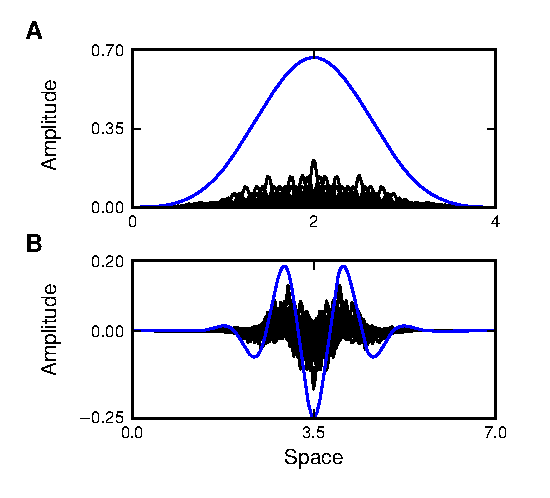
\includegraphics[scale=1]{./Graph/fig5.pdf}
 		\caption{{\bf The scaling and the wavelet function decomposition}. (\textbf{A}) The scaling function (blue) at $j=0$ is obtained using 625 scaling functions (black) at $j=4$. (\textbf{B}) The wavelet function (blue) at $j=0$ is obtained using 1250 scaling functions (black) at $j=4$.}
 	\label{fig:MRA-BasisDecomposition}
 \end{figure}  
In this paper, $4^{th}$ -- order cardinal B-spline scaling and wavelet functions are used, resulting in  $8^{th}$ and $12^{th}$ order B-spline functions when calculating Eq.~\eqref{eq:Lambdax} and Eq.~\eqref{eq:Uij} respectively  whose values at integer points are given in Table~\ref{table:MRA-BsplineatIntegerPoints}.
\begin {table}[t]
\begin{center}
	\begin{tabular}{lcccc}
	\hline \hline
	& $k$ & $3!N_{4}\left(k\right)$ & $7!N_{8}\left(k\right)$ & $11!N_{12}\left(k\right)$\\ 
	\hline 
	& 1 & $1$ & $1$ & $1$\\
	& 2 & $4$ & $120$ & $2,036$\\
	& 3 & $\space$ & $1,191$ & $152,637$\\
	& 4 & $\space$ & $2,416$ & $2,203,488$\\
	& 5 & $\space$ & $\space$ & $9,738,114$\\
	& 6 & $\space$ & $\space$ & $15,724,248$\\
	\hline \hline
	\end{tabular}
 \caption {{\bf Cardinal B-Splines at the knot sequence}. Table entries are calculated using Eq.~\eqref{eq:MRA-recursiveBsplineatintegerpoints} and can be also found in \citet{Goswami1999}.} 
 \label{table:MRA-BsplineatIntegerPoints}
 \end{center}
 \end {table}
\subsection{Frequency Analysis}\label{sec:freq_anal}
To determine the level of approximation in the model, $j$, detailed in the previous section, that is the number of basis functions required to reconstruct the field, $v_t(r)$, the frequency response of the B-spline function needs to be computed by applying the Fourier transform to Eq.~\eqref{eq:N1convolutions}. To proceed the Fourier transform of $N_1(r)$ is first calculated, 
\begin{align}\label{eq:MRA-N1Fouriertransform}
\mathcal F(N_1(r))&=\int_{-\infty}^{+\infty}N_1(r)\mathrm{exp}(-2\pi i \nu r)dr \nonumber \\
&=\int_{0}^{1} \mathrm{exp}(-2\pi i \nu r)dr \nonumber \\
&=\frac{1-\mathrm{exp}(-2\pi i \nu)}{2\pi i\nu},
\end{align}
where $i=\sqrt{-1}$. The convolution theorem states that the Fourier transform of the convolution of functions is equal to the product of their Fourier transforms. Therefore, taking Fourier transform of Eq.~\eqref{eq:N1convolutions} and substituting Eq.~\eqref{eq:MRA-N1Fouriertransform} for $\mathcal F(N_1(r)) $ yields
\begin{align}\label{eq:MRA-NmFouriertransform}
\mathcal F(N_m(r))=\left(\frac{1-\mathrm{exp}(-2\pi i \nu)}{2\pi i\nu}\right)^{m}.
\end{align}
The Fourier transform of the $m^{th}$ order B-spline allows the calculation of the spatial frequency response of the wavelets using Eq.~\eqref{eq:MRA-TwoScalepair2} giving
\begin{align}      
	  \mathcal{F}(\varphi_{m}\left(r\right)) &= \sum_{n=0}^{3m-2} \left[\mathbf q\right]_n \mathcal{F}\left(N_{m}\left(2r-n\right)\right) \nonumber\\
	&=\frac{1}{2}\left(\frac{1-\mathrm{exp}(-\pi i \nu)}{\pi i\nu}\right)^m~\sum_{n=0}^{3m-2} \left[\mathbf q\right]_n \mathrm{exp}(-\pi in\nu).\label{eq:MRA-Wavelettransform}
\end{align}
From Eq.~\eqref{eq:MRA-Wavelettransform} the frequency response of the wavelets and hence the level of approximation, $j$, can be determined. This way we choose wavelets up to level $j$ that can fully describe the spatial frequency contents of the underlying dynamics from the observed field.

\section{State and Parameter Estimation}
The aim of this section is to describe the joint state-parameter estimation method used in this study, the expectation maximization (EM) algorithm. Here we provide a general description of the algorithm and also discuss the specific formulation for MRAIDE framework. 

There exist many variations of state and parameter estimation methods for state-space models. The choice of algorithm is normally determined by the dimension of the system, whether the system is linear or nonlinear and whether or not the parameters are considered static or dynamic. Up to this point of the paper, we have not made any assumptions on any of these criteria for choosing an estimation algorithm. The MRAIDE neural field model formulation may be used in any of the above scenarios. 

To demonstrate the MRAIDE estimation framework we shall consider the parameters to be static and we shall also assume that the relationship between the mean membrane potential and the mean firing rate is predominantly linear. Note that there is a difference between forward and inverse modeling when making these assumptions. For example, by using a linear activation function in the estimator we are not assuming that there is necessarily a linear relationship between the membrane voltage and firing rate, but that the statistics of the neural masses fall within a linear operating region over the estimation time period. The major benefit of modeling the relationship between the mean membrane potential and firing rate is the ability to apply the EM algorithm. \dean{The loss in model accuracy may be offset estimation accuracy. }

It is important to point out there is no doubt that there will always be a mismatch between neural mass models and actual cortical tissue. Nevertheless, the simplifications used in formulating the equations enable the development of new methods for extracting information from electrophysiological data, that has the potential to influence the treatment of diseases such as epilepsy. The trade-off between parsimony and complexity is always difficult when considering neurodynamics and this is further complicated when using estimation algorithms that have huge computational demands with such high-dimensional systems.  

% The linearised activation function is 
% \begin{align}
% 	\hat{f}(v_t\left(\mathbf{r}\right)) &= f(v_0) + f'(v_0)(v_t\left(\mathbf{r}\right) - v_0) \\
% 	&= \frac{2 + \varsigma(v_t\left(\mathbf{r}\right) - v_0)}{4}. \label{eq:LinearActivationFunction} 
% \end{align}

By assuming a linear activation function of the form
\begin{equation}
	f(v_t(\mathbf{r})) = \varsigma v_t(\mathbf{r}),
\end{equation}
the state transition equation~\eqref{eq:ApproxDiscreteTimeModel4} simplifies to
\begin{equation}\label{eq:ApproxDiscreteTimeModel_Linear}
	\mathbf{x}_{t+1} = 
	\xi \mathbf{x}_t + 
	\varsigma T_s \mathbf{\Lambda}_{x}^{-1} \int_{\Omega}\boldsymbol\mu\left(\mathbf{r}\right)\int_\Omega { 
	    \boldsymbol\theta^\top\boldsymbol\lambda\left(\mathbf{r}-\mathbf{r}'\right)
	    \boldsymbol\mu^\top\left(\mathbf{r}'\right) 
	\, \mathrm{d}\mathbf{r}'\mathrm{d}\mathbf{r}} \mathbf{x}_t
	+ \mathbf{w}_t.
\end{equation}
Now we can further simplify the system by defining
\begin{align}
	\label{eq:Lambdatheta}
	 \mathbf{\Lambda}_{\theta} &\triangleq \int_{\Omega}\boldsymbol\mu\left(r\right) \int_\Omega { 
		   \boldsymbol\theta^\top\boldsymbol\lambda\left(r-r'\right)
		    \boldsymbol\mu^\top\left(r\right)\ \mathrm{d}r'\mathrm{d}r},
\end{align}
to give the state equation
\begin{equation}\label{eq:StateEquation}
 \mathbf x_{t+1} =\mathbf A(\boldsymbol \theta) \mathbf x_t+ \mathbf w_t,
\end{equation} 
with the parameterized transition matrix
\begin{equation}\label{eq:A_theta}
 \mathbf A(\boldsymbol \theta)= T_s\varsigma\mathbf{\Lambda}_{x}^{-1}\mathbf{\Lambda}_{\theta}+\xi\mathbf I.
\end{equation} 
The problem of joint state and parameter estimation for the state-space model given by Eq.~\eqref{eq:StateEquation} and Eq.~\eqref{eq:ReducedObservationEquation} can be formulated as 
\begin{equation}
	{\hat{\mathbf X},\hat{\boldsymbol\theta}}=\arg\max_{\mathbf X,\boldsymbol\theta}p(\mathbf Y;\boldsymbol\theta),
 \end{equation}  
where $\mathbf X$ and $\mathbf Y$ denote the entire sequences of the states and observations respectively, $\boldsymbol\theta$ is the parameter set and $p(\mathbf Y;\boldsymbol\theta)$ denotes the probability density function of the observations parameterized  by $\boldsymbol\theta$, known as the likelihood function. This dual estimation problem cannot be solved separately, as for the state estimation the knowledge of the system's parameters is required and for the parameter estimation the states of the system need to be known. One approach is to iteratively estimate the states and parameters of the system and monitor the convergence of the algorithm. A natural framework to perform this is the well known Expectation Maximization (EM) algorithm \citep{Dempster1977,Shumway2000} to infer both the parameter set and the states from the observations corresponding to the connectivity kernel, the neural field and electrophysiological data in our application. The EM algorithm is applicable  in two main situations:  first is when the observations are incomplete due to a faulty observation process or existing limitations and the second is when the direct maximization of the likelihood function is difficult but can be simplified by assuming the existence of an additional data referred to as hidden data \citep{Bilmes1998}, the weights of the field basis functions in this case. The EM algorithm, when used in the latter context \citep{Dewar2009}, yields the maximum likelihood kernel estimate, i.e.
\begin{equation}
	\boldsymbol\theta_{\text{ML}}=\arg\max_{\boldsymbol\theta}~p(\mathbf Y;\boldsymbol\theta),
 \end{equation}   
and the posterior distribution of the field over time.

Both the E and the M steps of the EM algorithm find increasingly tighter lower bounds on the likelihood of the parameters so that, at convergence, the maximum of the bound corresponds to the maximum of the likelihood. For state-space models, the E-step corresponds to the smoothing problem, which can be solved using the Rauch Tung Streibel (RTS) smoother \cite{RAUCH1965}. For the M-step, a lower bound on the likelihood function is constructed, where the steps needed
to compute the required quantities are very dependent on the particular application. This will be described in detail for our problem. 

In summary, to solve the joint state and parameter estimation for linear state-space models one can adapt the EM algorithm, solving the smoothing problem for the E-step and constructing and maximizing the lower bound in the M-step. A schematic representation of the EM algorithm is represented in Fig.~\ref{fig:EMBlockDiagram}. Note the algorithm can be initialized by either a random parameter set or a sequence of the random bounded state vectors. Here the latter is chosen as shown in the block diagram ensuring the resultant initial kernel estimate leads to a stable system.  
\begin{figure}[!t]
\centering
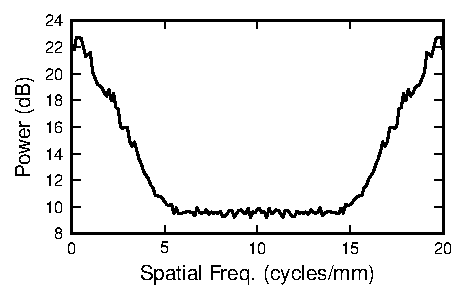
\includegraphics[scale=1]{./Graph/fig6.pdf}
\caption{{\bf Schematic of the EM algorithm}. The RTS smoother (E-step) and the maximization of the lower bound, $\mathcal Q(\boldsymbol \theta,\boldsymbol\theta')$, (M-step) are shown. The dashed box shows the iterative two step algorithm once it is initialized.}
\label{fig:EMBlockDiagram}
\end{figure}
\subsection{E-step}
As mentioned earlier, the E-step for state-space models is equivalent to the smoothing problem. We use the RTS smoother, given in Table~\ref{alg:MRA-RTS} for completeness, in order to infer the states of the system. The RTS smoother uses the Kalman filter \citep{Kalman1960} in forward pass (Steps~1 and 2 in Table~\ref{alg:MRA-RTS}), along with a backward iteration to calculate its outputs (Steps~3 and 4 in Table~\ref{alg:MRA-RTS}): smoothed states $\hat{\mathbf x}^b_t$ and covariances, $\mathbf P^b_t=\mathrm{cov}(\mathbf{x}_t)$. Following \cite{Gibsona2005}, an additional backwards recursion is also included (Step~5 in Table~\ref{alg:MRA-RTS})	to calculate cross-covariance matrix, $\mathbf M_t=\mathrm{cov}(\mathbf{x}_{t},\mathbf{x}_{t+1})$, which is also required in forming the lower bound to be maximized in the M-step. Note that the following quantities from the forward iteration should be stored when the RTS smoother is implemented: predicted and corrected estimates for both state estimates ($\hat{\mathbf{x}}_t^{f-}$, $\hat{\mathbf{x}}_t^{f}$) and covariance matrices ($\mathbf P_t^{f-}$,$\mathbf P_t^f$). Also, the final value of the Kalman gain, $\mathcal K_T$, should be stored in order to initialize the backward cross-covariance computation. 
\renewcommand{\arraystretch}{1.7}
\begin{table*}[!ht]
\begin{tabular}{|c|}\hline
\multicolumn{1}{|p{16cm}|}{\textbf{1.} Forward initialization} \\ 
$\hat{\mathbf x}_0, \mathbf P_0$ \\
\hline
\multicolumn{1}{|p{16cm}|}{\textbf{2.} Forward iteration: for $t\in\left\lbrace 0,\cdots,T-1\right\rbrace $, calculate the predicted state and the predicted covariance matrix } \\
$\hat{\mathbf x}_{t+1}^{f-}=\mathbf A \hat{\mathbf x}_{t}^{f}$  \\ 
$\mathbf P_{t+1}^{f-}=\mathbf A \mathbf P_{t}^{f}\mathbf A^{\top}+\boldsymbol\Sigma_e$  \\
\multicolumn{1}{|p{16cm}|}{Compute the filter gain, the filtered state and the filtered covariance matrix} \\
$\mathcal K_{t+1}=\mathbf P_{t +1}^{f-}\mathbf C ^\top(\mathbf C \mathbf P_{t +1}^{f-}\mathbf C ^\top+\boldsymbol \Sigma_{\varepsilon})^{-1}$\\
$\hat{\mathbf x}_{t+1}^{f}=\hat{\mathbf x}_{t+1}^{f-}+\mathcal K_{t+1}(\mathbf y_{t+1}-\mathbf C\hat{\mathbf x}_{t +1}^{f-})$\\
$\mathbf P_{t+1}^f=(\mathbf I - \mathcal K_{t+1}\mathbf C)\mathbf P_{t +1}^{f-}$\\
\hline
\multicolumn{1}{|p{16cm}|}{\textbf{3.} Backward initialization}\\
 $\mathbf P_T^b= \mathbf P_T^f, \quad \hat{\mathbf x}^b_T= \hat{\mathbf x}^f_T$\\
\hline
\multicolumn{1}{|p{16cm}|}{\textbf{4.} Backward iteration: for $t\in\left\lbrace T-1,\cdots,0\right\rbrace $ compute the smoother gain, the smoothed state and the smoothed covariance matrix}\\  
$\mathcal S_{t}=\mathbf P_{t}^{f}\mathbf A^{\top}\left[ \mathbf P_{t +1}^{f-}\right]^{-1}$ \\
 $\hat{\mathbf x}_t^b=\hat{\mathbf x}_t^f+\mathcal S_t(\hat{\mathbf x}_{t+1}^{b}-\hat{\mathbf x}_{t+1}^{f-})$ \\
 $\mathbf P_{t}^{b}=\mathbf P_{t}^{f}+\mathcal S_t(\mathbf P_{t+1}^{b}-\mathbf P_{t+1}^{f-})\mathcal S_t^\top$\\  
\hline
\multicolumn{1}{|p{16cm}|}{\textbf{5.} Compute the smoothed cross covariance matrix, initialization}\\
$\mathbf M_T=(\mathbf I-\mathcal K_T\mathbf C)\mathbf A\mathbf P_{T-1}^b$\\
\multicolumn{1}{|p{16cm}|}{For $t\in\left\lbrace T-1,\cdots,1\right\rbrace $ compute}\\
$\mathbf M_t= \mathbf P_t^{f}\mathcal S_{t-1}^{\top}+\mathcal S_{t}(\mathbf M_{t+1}-\mathbf A\mathbf P_t^{f} )\mathcal S_{t-1}^{\top}$\\
\hline
\end{tabular}
\caption{\textbf{Algorithm for the RTS smoother} This table shows the steps in the  Rauch-Tung-Striebel smoother algorithm. The lower bound, $\mathcal{Q}(\boldsymbol{\theta},\boldsymbol{\theta'})$, is maximized after each iteration to update the parameter estimates.}
\label{alg:MRA-RTS}
\end{table*}
\renewcommand{\arraystretch}{1}
 \subsection{M-step}
The lower bound on the log-likelihood function is given by the expectation of the complete (hidden and observable) data  log-likelihood \citep{Bishop2006} 
\begin{equation}\label{eq:Bishopbound}
	\mathcal Q(\boldsymbol \theta,\boldsymbol\theta')= \mathbf E_{\boldsymbol \theta'}\left[2\ln p(\mathbf X,\mathbf Y;\boldsymbol \theta)\right], 
\end{equation}
where $p(\mathbf X,\mathbf Y;\boldsymbol \theta)$ is the joint probability distribution of the states and the observations and $ \mathbf E_{\boldsymbol \theta'}\left[\cdot\right] $ denotes expectation taken with respect to the marginal distribution of the states conditioned on the observed field and the current estimate of the parameter set, $\boldsymbol\theta'$ i.e.  $p(\mathbf X\mid\mathbf Y;\boldsymbol \theta'$). Note that this is actually the smoother output which is obtained at the E-step.

For the linear state-space model given by Eqs.~\eqref{eq:StateEquation} and \eqref{eq:ReducedObservationEquation}, the bound defined by Eq.~\eqref{eq:Bishopbound} is a quadratic of the form (see \ref{ap:QDerivation} for derivation) 
\begin{equation}\label{eq:MRA-QCompact}
\mathcal Q\left(\boldsymbol \theta,\boldsymbol\theta'\right)=\beta+2T_s\varsigma\left(\boldsymbol\upsilon_0-\boldsymbol\upsilon_1\right)\boldsymbol\theta-T_s\varsigma\boldsymbol\theta^\top\boldsymbol\Upsilon\boldsymbol\theta,
\end{equation}
where $\beta$ is constant with respect to $\boldsymbol\theta$. Equation~\eqref{eq:MRA-QCompact} is maximum at
\begin{align}\label{eq:MRA-thetahat}
\boldsymbol \theta= \boldsymbol\Upsilon^{-\top}(\boldsymbol\upsilon_0-\boldsymbol\upsilon_1)^\top,
\end{align}
where
\begin{align}
\boldsymbol\upsilon_0&=\sum_{i,j=1}^{n_x}[\boldsymbol\Xi_0]_{i,j}[\boldsymbol\Gamma_1]_{j,i}\label{eq:epsilon0} \\
\boldsymbol\upsilon_1&=\xi\sum_{i,j=1}^{n_x}[\boldsymbol\Xi_1]_{i,j}[\boldsymbol\Gamma_1]^{j,i} \label{eq:epsilon1}\\
\boldsymbol\Upsilon&=T_s\varsigma\sum_{i,j=1}^{n_x}[\boldsymbol\Xi_1]_{i,j}[\boldsymbol\Gamma_2]^{j,i},\label{eq:Epsilon}
\end{align} 
where $[\cdot]_{p,q}$ denotes the $\left(p,q\right)$-element of the matrix, and $ [\cdot]^{p,q}$ denotes the $\left(p,q\right)$-block of the block matrix and where 
\begin{align}
\left[ \Gamma_1\right]^{j,i} &=\sum_{k=1}^{n_x}\left[ \boldsymbol\Sigma_w^{-1}\boldsymbol\Lambda_x^{-1}\right]_{jk} \left[ \mathbf U\right]^{k,i},\\
\left[ \Gamma_2\right] ^{j,i}&=\sum_{k,m=1}^{n_x}[\mathbf U^{\top}]^{jk} \left[\boldsymbol\Lambda_x^{-1}\boldsymbol\Sigma_w^{-1}\boldsymbol\Lambda_x^{-1} \right]_{km}[\mathbf U]^{mi}.
\end{align}
Each $ 1 \times n_{\theta}$ block of the $n_x \times n_x n_{\theta}$ block matrix $\mathbf U$ is 
\begin{align}\label{eq:Uij}
\left[ \mathbf U\right] ^{k,i}&=\int_{\boldsymbol \Omega}\left[\boldsymbol\mu(r) \right]_k \left[\int_{\boldsymbol\Omega} \boldsymbol\mu\left(r'\right)\boldsymbol \lambda^\top \left(r-r'\right) \mathrm{d}r'\right]_{i:} \mathrm{d}r,
\end{align}
where $[\cdot]_{i:} $ denotes the $i^{th}$ row. The matrices $\boldsymbol\Xi_0$ and $\boldsymbol\Xi_1$ in Eqs.~\eqref{eq:epsilon0}-\eqref{eq:Epsilon} are calculated using the RTS smoother outputs: $\hat{\mathbf x}_t$, covariance, $\mathbf P_t^b$, and cross-covariance matrix, $\mathbf M_t$ \citep{Gibsona2005}, 
\begin{align}
\boldsymbol\Xi_0&=\sum_{t=0}^{T-1}\left(\mathbf M_{t+1}+\mathbf{\hat x}_t\mathbf{\hat x}_{t+1}^\top\right) \label{eq:Xi0} \\
 \boldsymbol\Xi_1&=\sum_{t=0}^{T-1}\left(\mathbf P_t+\mathbf{\hat x}_t\mathbf{\hat x}_t^\top\right).  \label{eq:Xi1}
\end{align} 
The algorithm has two steps: the E-step, which computes $\boldsymbol\Xi_0$ and $\boldsymbol\Xi_1$ based on the most recent parameter estimates using the RTS smoother, and the M-step, which updates the parameter estimates by computing the (analytic) maximum of $Q(\boldsymbol\theta,\boldsymbol\theta')$. The EM algorithm iterates between these two steps until the parameter estimates converge. A summary of the joint state parameter estimation is given in Table~\ref{alg:EMsteps}.   
\subsection{Stopping rule}
The stopping criterion is usually associated with either the change in the parameter estimates or the log-likelihood variation \citep{McLachlan1997}. The stopping rule adopted herein is
\begin{equation}
 \left(\parallel \mathbf{A} \parallel_{F}^{(i)}-\parallel \mathbf{A} \parallel_{F}^{(i-1)}\right)<\epsilon,
 \end{equation}
 where $\epsilon$ is a threshold value and $\parallel \mathbf{A} \parallel_{F}^{(i)}$ and $ \parallel \mathbf{A} \parallel_{F}^{(i-1)}$ are the Frobenius norms  of the successive estimates of $\mathbf{A} $ matrices which is defined by \citet{Meyer2000}
 \begin{equation}
  \parallel \mathbf{A} \parallel_{F}=\sqrt{\sum_{i,j=1}^{n_x}\mid a_{i,j} \mid^2}=\sqrt{\mathrm{tr} (\mathbf A^{\top}\mathbf A)}.
 \end{equation}
\subsection{Computational complexity} 
All $n_x^2$ blocks of $\mathbf U$, $\boldsymbol\Gamma_1$ and $\boldsymbol\Gamma_2$  can be computed as a one-off before the commencement of the EM iterations, which increases the speed of the M-step significantly compared to the implementation of \citet{Dewar2009}. The complexity of each step of the algorithm is summarized in Table~\ref{table:MRA-ComputationalComplexity} where for ease of comparison the computational complexity of the method of \citet{Dewar2009} is also identified. It can be seen from the table that the state dimension is an important factor at each iteration of the estimation algorithm, emphasizing the advantage of the proposed algorithm compared to the method proposed in \citet{Dewar2009}. This also suggests the use of an efficient algorithm to choose the minimum number of basis functions (states of the system) while achieving the desired details of the underlying field.  
\begin {table}
\begin{center}
\scalebox{1}{\begin{tabular}{lllc}
\hline \hline
Variable &Equation&Order&Order obtained from \citet{Dewar2009}\\ \hline\\
$\Xi_0, \Xi_1$&Eqs.~\eqref{eq:Xi0} and \eqref{eq:Xi1}&$O(Tn_x^2)$& \----\\
$\boldsymbol\upsilon_0, \boldsymbol\upsilon_1$&Eqs.~\eqref{eq:epsilon0} and \eqref{eq:epsilon1} &$O(n_x^2n_{\theta})$ &$O(n_x^2n_{\theta})+O(n_x^3)$ \\
$\boldsymbol\Upsilon$&Eq.~\eqref{eq:Epsilon}&$O(n_x^2n_{\theta}^2)$&$O(n_x^4n_{\theta}^2)$\\
$\mathbf A(\boldsymbol\theta)$&Eq.~\eqref{eq:A_theta}&$O(n_x^3)$&\----\\
$\boldsymbol\Lambda_{\theta}$&Eq.~\eqref{eq:LambdaThetaElements}&$O(n_x^2n_{\theta})$&\----\\
$\hat{\boldsymbol\theta} $&Eq.~\eqref{eq:MRA-thetahat}&$O(n_{\theta}^3)$&\----\\
\hline \hline
\end{tabular}}
 \caption {{\bf The Computational complexity of the estimation algorithm}. A comparison between the algorithm proposed herein and that of \citet{Dewar2009} is also provided. "\----'' indicate equal complexities for both algorithms.} 
\label{table:MRA-ComputationalComplexity}
\end{center}
\end {table} 
%%%%%%%%%%%%%%%%%%%%%%%%%%%%%%%%%%%%%%%%%%%%%%%%%%%%%%%%%%%%%%%%%%%%%%%%%%%%%
\renewcommand{\arraystretch}{1.7}
\begin{table*}[!ht]
\begin{tabular}{|c|}\hline
\multicolumn{1}{|p{16cm}|}{\textbf{1.} Initialization:  } \\ 
\multicolumn{1}{|p{16cm}|}{Choose a bounded random state vector sequence and choose large values for $\mathbf P_t$ and $\mathbf M_t$} \\
\multicolumn{1}{|p{16cm}|}{Compute} \\
$\mathbf{\Lambda}_{x}=\int_{\Omega}\boldsymbol{\mu}\left(r\right)\boldsymbol{\mu}^\top\left(r\right) \mathrm{d}r$\\
\multicolumn{1}{|p{16cm}|}{Compute all the $n^2_x$ blocks of block matrices $\mathbf U$, $\Gamma_1$ and  $\Gamma_2$ using} \\
$\left[ \mathbf U\right] ^{k,i}=\int_{\boldsymbol \Omega}\left[\boldsymbol\mu(r) \right]_k \left[\int_{\boldsymbol\Omega} \boldsymbol\mu\left(r'\right)\boldsymbol \lambda^\top \left(r-r'\right) dr'\right]_{i:} dr$\\
$\left[ \Gamma_1\right]^{j,i} =\sum_{k=1}^{n_x}\left[ \boldsymbol\Sigma_w^{-1}\boldsymbol\Lambda_x^{-1}\right]_{jk} \left[ \mathbf U\right]^{k,i}$\\
$\left[ \Gamma_2\right] ^{j,i}=\sum_{k,m=1}^{n_x}[\mathbf U^{\top}]^{jk} \left[\boldsymbol\Lambda_x^{-1}\boldsymbol\Sigma_w^{-1}\boldsymbol\Lambda_x^{-1} \right]_{km}[\mathbf U]^{mi}$\\
\hline
\multicolumn{1}{|p{16cm}|}{\textbf{2.} Estimate the connectivity kernel parameters} \\
$\boldsymbol\Xi_0=\sum_{t=0}^{T-1}\left(\mathbf M_{t+1}+\mathbf{\hat x}_t\mathbf{\hat x}_{t+1}^\top\right)$\\
$\boldsymbol\Xi_1=\sum_{t=0}^{T-1}\left(\mathbf P_t+\mathbf{\hat x}_t\mathbf{\hat x}_t^\top\right)$\\
$\boldsymbol\upsilon_0=\sum_{i,j=1}^{n_x}[\boldsymbol\Xi_0]_{i,j}[\boldsymbol\Gamma_1]_{j,i}$\\
$\boldsymbol\upsilon_1=\xi\sum_{i,j=1}^{n_x}[\boldsymbol\Xi_1]_{i,j}[\boldsymbol\Gamma_1]^{j,i}$\\
$\boldsymbol\Upsilon=T_s\varsigma\sum_{i,j=1}^{n_x}[\boldsymbol\Xi_1]_{i,j}[\boldsymbol\Gamma_2]^{j,i}$\\
$\boldsymbol \theta= \boldsymbol\Upsilon^{-\top}(\boldsymbol\upsilon_0-\boldsymbol\upsilon_1)^\top$\\
\hline
\multicolumn{1}{|p{16cm}|}{\textbf{3.} Form a state-space model}\\
\multicolumn{1}{|p{16cm}|}{Compute all $n_x^2$ elements of $\boldsymbol\Lambda_{\theta}$ using} \\
$\left[ \boldsymbol\Lambda_{\theta}\right] _{k,i}=\left[ \mathbf U\right]^{k,i}\boldsymbol\theta$\\
\multicolumn{1}{|p{16cm}|}{Compute transition matrix $\mathbf A(\boldsymbol\theta)$ } \\
$\mathbf A(\boldsymbol \theta) = T_s\varsigma\mathbf{\Lambda}_{x}^{-1}\mathbf{\Lambda}_{\theta}+\xi\mathbf I$\\
\hline
\multicolumn{1}{|p{16cm}|}{\textbf{4.} Compute the smoothed state $\hat{\mathbf x}_t^b$, the smoothed covariance,$\mathbf P^b_t$ and cross-covariance $\mathbf M_t$ for $t\in\left\lbrace 0,\cdots,T\right\rbrace $ using the RTS smoother given in Table~\ref{alg:MRA-RTS}.}\\  
\hline
\multicolumn{1}{|p{16cm}|}{\textbf{5.} Convergence: go back to Step~2 unless }\\
$ \left(\parallel \mathbf{A} \parallel_{F}^{(i)}-\parallel \mathbf{A} \parallel_{F}^{(i-1)}\right)<\epsilon$\\
\hline
\end{tabular}
\caption{\textbf{State and parameter estimation for the MRAIDE model.} This table shows the steps for the joint state and parameter estimation using the EM based algorithm.}
\label{alg:EMsteps}
\end{table*}
\renewcommand{\arraystretch}{1}
%%%%%%%%%%%%%%%%%%%%%%%%%%%%%%%%%%%%%%%%%%%%%%%%%%%%%%%%%%%%%%%%%%%%%%%%%%%%%%
\section{Results}\label{sec:MRA-results}
To demonstrate the performance of the MRAIDE estimation framework, data was generated synthetically  using Eqs.~\eqref{eq:DiscreteTimeModel} and \eqref{eq:ObservationEquation}, allowing a comparison between true and estimated parameters. In doing so, the membrane time constant was set to $\tau = 10$~ms \citep{David2003}, and the sampling time was chosen ten times faster \citep{Stephan2008}, i.e. $T_s = 1$~ms, ensuring the discrepancy between the continuous neural field model and its discrete approximation is small. The connectivity kernel used for data generation composed of two B-spline scaling functions at $j=0$ and $j=1$ forming a compact support Mexican hat shape 
\begin{equation}\label{eq:ConnectivityKernelForData}
	w(r-r')=\theta_1\times N_{4;1,2}(r-r')+\theta_2\times N_{4;0,2}(r-r'),
\end{equation}
with $\theta_1=200$ and $\theta_2=-100$. This is depicted in Fig.~\ref{fig:KernelEstimate}(A).

Two different experiments were designed to test the framework. In the first one, 200 realizations of 1 second of data were used, where the field disturbance, $e_t$, and the observation noise, $\boldsymbol\epsilon_t$, were regenerated each run. This way the net shape of the connectivity kernel could be formed by averaging over the parameters estimates from each realization. \dean{the frequency response of the observed field used to decide on the level...} In the second experiment, a single data set was generated and the field estimations are compared for five state-space models, each accounting up to a certain level of approximation, i.e. $j=0$ to $j=4$. All parameters for the model are given in Table~\ref{tab:Parameters}.

For each of the experiments, the estimation was applied to the final 900~ms, allowing the forward model's dynamics to stabilize from the initial conditions. The initial state, parameters and the support of the connectivity kernel were unknown to the estimator. The observation noise was set to $\boldsymbol\Sigma_{\epsilon}=0.1 \times \mathbf{I}_{n_y}$ and the disturbance covariance function was set to $\eta(r-r') = \sigma_d\times\varphi_{4;3,2}(r-r')$ (B-spline, $j=3$) with $\sigma_d=0.53$.  The firing rate slope, $\varsigma$ was set to $0.56~mV^{-1}$ \citep{Wendling2005}. The observation kernel was modeled using a B-spline function, with a width of 0.08~mm at half the maximum amplitude where the distance between adjacent sensors was $0.05$~mm, resulting into $n_y = 161$ observations. The choice of B-spline function to model the observation kernel is justified by the experiment performed in \citep{Freestone2011}. The spacing and bandwidth of the sensors allowed the full spatial bandwidth of the field to be observed.  With this number of observations, the estimation problem was well-posed, i.e. the number of states, $n_x < n_y$ at each level of the decomposition. This is because the scaling functions are orthogonal to the wavelets at the same and higher levels of decomposition, and  the wavelets are orthogonal to each other across different scales (see Eqs.~\eqref{eq:MRA-PsiPsiOrthogonality} and \eqref{eq:MRA-PhiPsiOrthogonality}).
\begin{table*}[!ht]
\begin{tabular}{|c|l|c|l|}
	\hline
	\textbf{Symbol} & \textbf{Quantity} & \textbf{Value} & \textbf{Units}\\
	\hline
	\multicolumn{4}{|c|}{\emph{Domain and indices}}\\
	\hline
	$\Delta$ & spatial discretisation step & 0.01 & mm \\
	$T_s$ & time step & $0.001$ & s\\
	$T$ & number of time steps used in estimation & 900 & n.a.\\
	\hline 
\multicolumn{4}{|c|}{\emph{Model}}\\
	\hline
	$\tau$ & membrane time constant & 0.01 & s$^{-1}$ \\
	$\varsigma$ & slope of sigmoidal activation function & 0.56 \citep{Wendling2005} & mV$^{-1}$.spike.s$^{-1}$\\
	$\boldsymbol{\theta}$ & vector of connectivity kernel parameters (data generation) & $\left[\begin{array}{cc}
	200 & -100
	\end{array}
	\right]^{\top}$ & mV.spike$^{-1}$\\
	%$\sigma_{\psi_{1}}, \sigma_{\psi_{2}}, \sigma_{\psi_{3}}$ & connectivity kernel width parameters & 1.8, 2.4, 6 & mm\\
	$n_y$ & number of sensors & 161 & n.a.\\ 
	$\Delta_y$ & distance between adjacent sensors & 0.05 & mm\\
	$\sigma_{m}$ & observation kernel full width at half maximum & 0.08 & mm \\
	$\Sigma_{\varepsilon}$ & observation noise variance & $0.1 \times I_{n_y}$ & mm$^2$ \\
	$\sigma_{\eta}$& disturbance covariance function full width at half maximum & 0.18 & mm\\
	$\sigma_{d}$ & disturbance variance & 0.53 & mV \\
	\hline 
	\multicolumn{4}{|c|}{\emph{Reduced Model}}\\
	\hline
	$n_x$ & number of field basis functions&& n.a.\\
	$   $ &Experiment~I&131&\\
	$   $ &Experiment~II&17, 33, 65, 131, 263&\\ 
	\hline 
	\multicolumn{4}{|c|}{\emph{Estimation}}\\ 
	\hline
	$n_{\theta}$&number of connectivity kernel basis functions for estimation&25&n.a.\\
	\hline 
\end{tabular}
\caption{\textbf{Parameters.} Parameters for the neural field model and the reduced model and the estimation procedure.}
\label{tab:Parameters}
\end{table*} 
\subsection{Experiment I}
The spatial frequency response of the observed field was used to specify the level of decomposition required to represent the field using the wavelets. This is shown in Fig.~\ref{fig:ObservationFrequencyResponce} where the graph obtained by averaging the spectral power of the spatial frequency (over time) from the observations \citep{Scerri2009}. The spatial bandwidths of wavelets were calculated analytically using Eq.~\eqref{eq:MRA-Wavelettransform}. The result suggested that wavelets up to level $j=3$ (with the bandwidth $\approx[5,8]$ cycles/mm) can represent the significant spatial characteristics of the field which yields $n_x = 131$ states, corresponding to 9 scaling functions for $j=0$ and 8, 16, 32 and 66 wavelet functions, respectively for $j=0$, $j=1$, $j=2$ and $j=3$. 
\begin{figure}[!t]
 	\centering
 		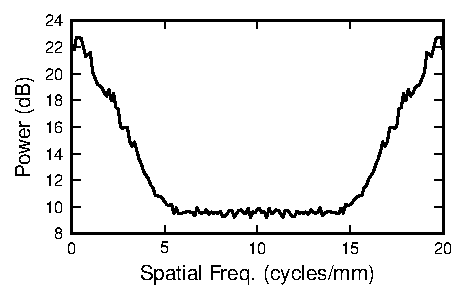
\includegraphics[scale=1]{./Graph/fig7.pdf}
 		\caption{{\bf Spatial frequency analysis}. The average (over time) power in dB of the spatial frequency of the observations.}  
\label{fig:ObservationFrequencyResponce} 
 \end{figure}

The EM algorithm was allowed to run until a maximum number of 20 iterations was reached, though typically the change in the transition matrix Frobenius norm dropped below $10^{-6}$ after less than 10 iterations. The rate of convergence of the EM based algorithm is depicted in Fig.~\ref{fig:MRA-Convergence}. 
\begin{figure}[t]
 	\centering
 		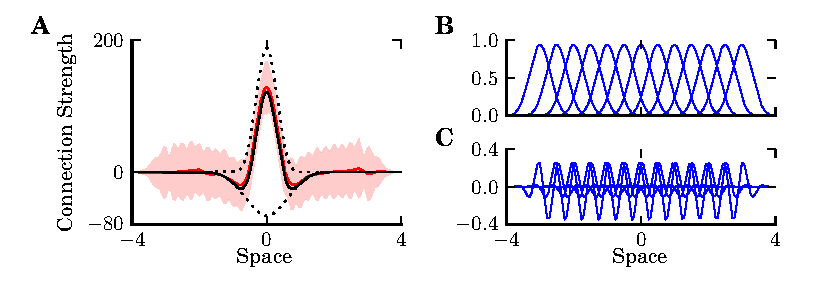
\includegraphics[scale=1]{./Graph/fig8.pdf}
 		\caption{{\bf Convergence of the EM based algorithm}. Representative plot of
the $\mathbf A(\boldsymbol\theta)$ Frobenius norm vs iterations of EM based algorithm. The change in the stopping criterion falls below $10^{-6}$ after less than 10 iterations.} 
\label{fig:MRA-Convergence}  
 \end{figure}     
% The spatial cutoff frequency of the observed field was used to specify the level of decomposition required to represent the field using the wavelets. Using an oversampling parameter of 5, the cutoff spatial frequency was $\nu_{cy} \approx 6.9 $ cycles/mm, obtained by averaging the spectral power of the spatial frequency (over time) from the observations \cite{Scerri2009}. Therefore, wavelets up to level $j=3$ (with the bandwidth $\approx[5,8]$ cycles/mm) can represent the significant spatial characteristics of the field, yielding $n_x = 131$ states. 
The actual connectivity kernel and the decomposition is plotted in Fig.~\ref{fig:KernelEstimate}(A). No assumptions where made about the shape of the kernel. The reconstructed kernel is in good accordance with the actual kernel, where the actual kernel lies inside the confidence interval. The large standard deviation is due to the high number of parameters need to be estimated. The small error in the estimate is attributed to the MRA of the system used to form the estimator. Fig.~\ref{fig:KernelEstimate}(B) and (C) illustrate the kernel scaling and wavelet functions, respectively. A total number of 25 basis functions were used to reconstruct the kernel, comprising 13 and 12 scaling and wavelet functions at $j=1$, respectively. 
\begin{figure}[!t]  
 \centering
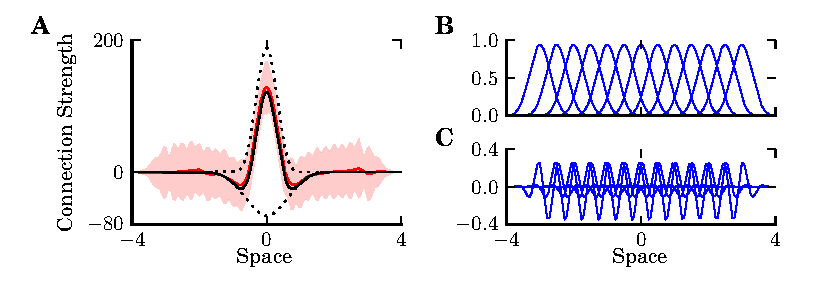
\includegraphics{./Graph/fig9.pdf}
\caption{ {\bf Connectivity kernel estimate}. (\textbf{A}) The actual kernel and its components are shown by solid and dashed black lines, respectively. The mean kernel estimates over 200 realizations and confidence interval are shown by the red line and red shaded region ($\pm2$ std.). (\textbf{B},\textbf{C}) Kernel scaling and wavelets functions, respectively, at $j=1$ used in the estimation algorithm.}
\label{fig:KernelEstimate}
\end{figure}

One snap shot of the field reconstruction, at different levels of approximation is given in Fig.~\ref{fig:FieldEstimates100}, showing small discrepancy between the actual and estimated field at $j=3$. From this figure, it can be observed that the overall trend of the underlying field can be also captured at the coarser levels.
\begin{figure}[!t]
\centering
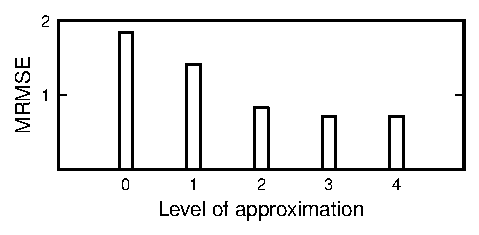
\includegraphics{./Graph/fig10.pdf}
\caption{ {\bf Examples of the actual and estimated neural fields for experiment I}. Actual (grey) and estimated (black) neural fields at a single time instant for different spatial resolutions. (\textbf{A}) $j=0$, $n_x=17$. (\textbf{B}) $j=1$, $n_x=33$. (\textbf{C}) $j=2$, $n_x=65$. (\textbf{D}) $j=3$, $n_x=131$.}
% (\textbf{e}) $j=4$, $n_x=263$.
\label{fig:FieldEstimates100}
\end{figure}
\subsection{Experiment II}
To study the performance of different models with various MRA capabilities, a single realization was obtained using Eqs.~\eqref{eq:DiscreteTimeModel} and \eqref{eq:ObservationEquation} under the same circumstances of the previous experiment. The generated data set was then employed to estimate the underlying field and the connectivity kernel parameters using different state-space models, $j=0$ up to $j=4$. The RMSE of the field estimation for different models is shown in Fig.~\ref{fig:RMSE}. By increasing the value of $j$, error in the estimation decreases and converges to a steady value of 0.71, confirming that the model with $j=3$ is in fact adequate to capture the dynamics of the underlying field. The spatiotemporal characteristics of the reconstructed fields (A-E) along with the actual field (F)  are shown in Fig.~\ref{fig:FieldEstimation}. The experiment was performed several times and the results were consistent over each run.
 \begin{figure}[!t]	 
 	\centering
 		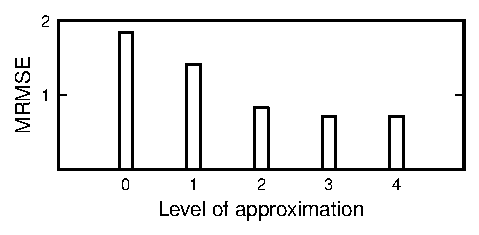
\includegraphics[scale=1]{./Graph/fig11.pdf}
 		\caption{{\bf Error in the field reconstruction for experiment II}. The mean (over time) of average (over space) RMSE of the estimated field of state-space models with different MRA capabilities. $j=0$, $RMSE = 1.83$; $j=1$, $RMSE = 1.41$; $j=2$, $RMSE = 0.83$; $j=3$, $RMSE = 0.71$; $j=4$, $RMSE=0.71$}
\label{fig:RMSE}
 \end{figure} 
\begin{figure}[t]
	\centering
		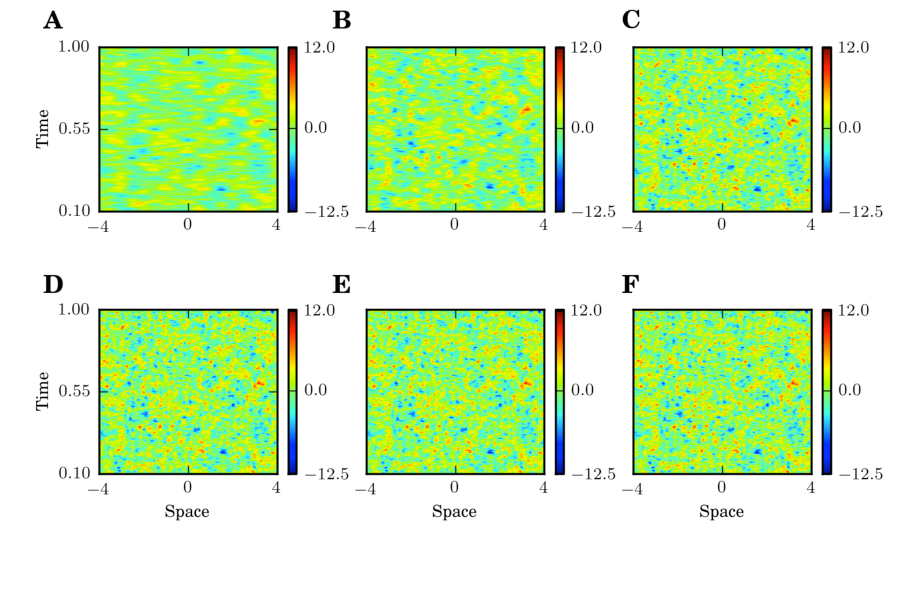
\includegraphics[scale=1]{./Graph/fig12.pdf}
	\caption{{\bf Actual and estimated spatiotemporal neural field using state-space models with different MRA capabilities}. (\textbf{A}) The reconstructed field of the reduced model using wavelet upto $j=0$ with $n_x=17$. (\textbf{B}) The reconstructed field using wavelets upto $j=1$ with $n_x=33$. (\textbf{C}) The reconstructed field  using wavelets upto $j=2$ with $n_x=65$. (\textbf{D}) The reconstructed field using wavelets upto $j=3$ with $n_x=131$. (\textbf{E}) The reconstructed field using wavelets upto $j=4$ with $n_x=263$. (\textbf{F}) The actual field.} 
\label{fig:FieldEstimation}
\end{figure}
% \caption{The actual connectivity kernel is shown with the black solid line. The estimated kernel and confidence interval is shown by the red line and red shaded region ($\pm2$ std.). The 7 weighted kernel basis functions are shown by the black dashed lines.}
\section{Discussion}
In this paper, we have presented a novel model-based framework for estimating cortical dynamics from electrophysiological measurements. The novel and key developments of the paper include the multi-resolution finite element model representation of the neural field, and the estimator for an intracortical connectivity kernel with an arbitrary shape. This work is significant, as the ability to create patient specific neural field models has the potential to contribute to our understanding and improve treatment of diseases resulting from abnormal neurodynamics, such as epilepsy. Other groups have previously highlighted the importance of a multi-resolution approach in neural field modeling. It is thought that the dynamics and connectivity structure differs at different spatial scales~\citep{Qubbaj2009,Breakspear2005,Schultze-Kraft2010}. %\dean{This is a test to see if we can fit something about Breaky's paper in here. It would be nice to slot something in here because he used wavelets.} 

For a larger space, or in a case where the connectivity kernel decomposition comprises of  many scale levels, the number of parameters to be estimated increases significantly. One solution to this problem could be expectation-conditional maximization (ECM) \citep{Meng1993,Meng1994}, which replaces the M-step by a series of computationally simplified conditional maximization (CM) steps. The ECM is a class of generalized EM (GEM)  algorithms in which the $\mathcal{Q}$-function is increased rather than being maximized \citep{Fessler1994}. For systems with a high number of states, the ensemble Kalman smoother (EnKS) \citep{Evensen2003,Evensen2009a,Evensen2009} provides an alternative to the RTS smoother used in this work. The EnKS is a sequential Monte Carlo (MC) method where the state covariance matrix is approximated by a large stochastic ensemble of model states, thus alleviating computational load due to the storage and forward integration of the state covariance matrix. However, combining the EnKS with the EM algorithm suffers from the loss of monotonicity property --- increase in the likelihood function--- as MC error will be introduced at the E-step.

Typically, a sequence of likelihood values will converge to a stationary point i.e. global (local) maximum or a saddle point. If the sequence of the EM is trapped in a local maximum or a saddle point, a small random perturbation diverges the algorithm from such stationary values \citep{McLachlan1997}. In general, convergence of the EM algorithm to any stationary point depends on the initialization. In the examples presented in this paper, a bounded sequence of the state vectors was used to initialize the algorithm, which gave a satisfactory convergence and good state and parameter estimations.


The MRAIDE approach is not limited to neural fields; the framework can be applied to modeling other multi-resolution spatiotemporal dynamical systems such as weather systems, ecological systems, and others~\citep{Wikle2002,Xu2005}. 
% \ken{meteorology [76, 88, 94, 222, 232], epidemiology [123, 137, 218], physics [32, 85, 129, 231], environmental science [45, 87, 183, 204] and economics [31, 48, 165]. (This is copy and paste from my thesis ... parham I'll get you the references later)}. \parham{Mike,Ken: can add to this list?}\mike{While I love this kind of thing for a review, I'm not sure we have space for this kind of thing? Also it's not terribly specific. I think it's better to stick to how it has the potential to model brains in a manner that rocks, rather than loosely saying it could be applied to any spatiotemporal system, i.e. literally everything.}

  % \mike{The framework makes two key assumptions about the cortex: a linear activation function and stationary dynamics. Our main aim for this framework in the future is to relax these assumptions using the multi-resolution decomposition. While the decomposition itself holds, efficiently performing nonlinear smoothing in the much larger state space remains a challenge. Additional avenues for future work include extending the model to capture a second order synaptic response kernel, and time delays \parham{at lower spatial resolutions}.  The estimation techniques should also be extended to deal with spatial and temporal heterogeneity in the kernel. Finally, the majority of our current work involves applying this framework to collected data, primarily for the use of seizure detection and mitigation.}

% In order to apply the framework to real data some assumptions must be made. A critical assumption is that the model provides an apt description of the cortical dynamics.

To demonstrate MRAIDE framework, an assumption was made where the firing rate behaves linearly. The implementation of the framework in the nonlinear case can be addressed as future work. Another future avenue would be the modification of the estimation framework to perform efficiently at higher dimensions. The reconstruction of the neural field requires $2^n-1$ wavelets, where $n$ is the dimension of the space. For example a two-dimensional MRA can be implemented using 2-D scaling and wavelet functions built up using the tensor-product approach \citep{Meyer1992}. In this case three wavelet functions are required to  extract fine features of the field at vertical, horizontal and diagonal orientations. The formulations provided in this paper can be easily extended to two dimensions. However, the computational load of the estimation algorithm will be significant. It is important to investigate methods for choosing basis functions to balance the complexity with the reconstruction capability of the model.
 
The authors acknowledge that there is, and will always be, a discrepancy between the model and cortex. Nevertheless, the model-based framework proposed in this paper may enable meaningful state tracking and connectivity estimation. The key development is the multi-resolution decomposition forming the state-space model. While the decomposition holds for more sophisticated models, efficiently performing nonlinear smoothing in the large state-space remains a challenge. 

Additional extension for future work include extending the model to capture a second order synaptic response kernel, The second-order postsynaptic kernel proposed in \citet{VanRotterdam1982} leads to dynamics that are more reminiscent to real postsynaptic potentials. Another extension of this framework is the inclusion of finite distant-dependent action potential propagation velocity into the parametric neural field equations. In small networks the delays via propagation can be neglected. However, delays must be accounted for in large scale networks. For instance, it is shown by \citet{Ghosh2008} that inclusion of time delays arising from propagation along connecting \parham{fibres} are essential for the fluctuations to be appeared in the default networks. Finally, future work should be directed towards applying and validating the framework on real data.

\newpage
\appendix
\section{Inner product of two B-spline scaling functions}\label{ap:InnerProductOfBsplines}
In this section, an analytic formula is derived for the inner product of two B-spline scaling functions. Consider two B-spline scaling functions of order $m$ and $m'$. The support of $N_m\left(s\right)$ is $\left[ 0,m\right]$ and  is symmetric with respect to $r=\frac{m}{2}$, i.e.
\begin{align}\label{eq:APP-SymmetrySplieEq}
 N_{m}\left(\frac{m}{2}+r\right)=N_{m}\left(\frac{m}{2}-r\right).
\end{align}
A direct consequence of Eq.~\eqref{eq:APP-SymmetrySplieEq} is 
\begin{align}
 N_{m}\left(r\right)=N_{m}\left(m-r\right).
\end{align}
Therefore
\begin{align}
\int_{-\infty}^{+\infty}N_{m}\left(r-l_{1}\right)N_{m'}\left(r-l_{2}\right)dr&=\int_{-\infty}^{+\infty}N_{m}\left(m-r+l_{1}\right)N_{m'}\left(r-l_{2}\right)dr \nonumber \\
&=\int_{-\infty}^{+\infty}N_{m}\left(m+l_{1}-l_{2}-u\right)N_{m'}\left(u\right)du \nonumber \\
&=\left(N_m \ast N_{m'}\right) \left(m+l_{1}-l_{2}\right) \nonumber \\
&=N_{m+m'}\left(m+l_{1}-l_{2}\right) \nonumber \\
&=N_{m+m'}\left(m'+l_{2}-l_{1}\right).
\end{align}
\section{Scaling function expansion}\label{ap:Induction}  
In this appendix we show by induction that how the scaling function at $j=0$ can be written in terms of the scaling function at level $j$. For $n_1$ in  Eq.~\eqref{eq:MRA-ConvertingFormulaForscalingFunctions} we have
\begin{align}
 N_{m}\left(r\right)&=\sum_{n_1=0}^{m} \left[\mathbf p\right]_{n_1} N_{m}\left(2r-n_1\right) \label{eq:App-TwoScalepair1},
  \end{align}
which clearly holds from two-scale relation pair (see Eq.~\eqref{eq:MRA-TwoScalepair1}). Now assuming Eq.~\eqref{eq:MRA-ConvertingFormulaForscalingFunctions} for $n_{j-1}$ we can write 
\begin{align}\label{eq:app-ConvertingFormulaForscalingFunctions}
 &N_m(r)=\nonumber \\
&\sum_{n_1,n_2, \dots n_{j-1}=0}^{m}\left[\mathbf p\right]_{n_1} \left[\mathbf p\right]_{n_2}\dots \left[\mathbf p\right]_{n_{j-1}}N_m(2^{j-1}r-k_{n_1,n_2, \dots, n_{j-1}}),
\end{align}
in which $N_m(2^{j-1}r-k_{n_1,n_2, \dots, n_{j-1}})$ can be written in terms of $N_m(2^{j}r)$ as
\begin{align}\label{eq:AppendixNj-1intermsofNj}
 N_m(2^{j-1}r-k_{n_1,n_2, \dots, n_{j-1}})&=\sum_{n_j=0}^m \left[\mathbf p\right]_{n_j}N_m(2^jr-2\times k_{n_1,n_2, \dots, n_{j-1}}-n_j)\nonumber \\
&=\sum_{n_j=0}^m \left[\mathbf p\right]_{n_j}N_m(2^jr- k_{n_1,n_2, \dots, n_{j}}).
\end{align}
Substituting Eq.~\eqref{eq:AppendixNj-1intermsofNj} into Eq.~\eqref{eq:app-ConvertingFormulaForscalingFunctions} completes the proof. 

%\section{Lower bound on likelihood function}\label{ap:Lowerbound}
%A derivation of the lower bound on the likelihood function that is based on \citet{Bishop2006} is provided in this Appendix. We want to maximize the likelihood function, 
%\begin{equation}
 %p(\mathbf Y;\boldsymbol\theta)=\int_{\mathbf X}p(\mathbf X,\mathbf Y;\boldsymbol\theta)\mathrm{d}\mathbf X,
%\end{equation}
%which is difficult to perform directly. Maximizing the likelihood in terms of the parameter set is equivalent to the log-likelihood maximization, as both the likelihood and log-likelihood functions share the same maximizer due to the monotonicity of the logarithm function. For any choice of distribution defined over the hidden variables, $q(\mathbf X)$, the following decomposition holds
%\begin{equation}\label{eq:EM-loglikelihooddecomposition}
 %\ln~p(\mathbf Y;\boldsymbol\theta)=\mathcal{L}(q,\boldsymbol\theta)+\mathrm{KL}(q\parallel p),
%\end{equation}
%where
%\begin{align}
 %\mathcal{L}(q,\boldsymbol\theta)&=\int_{\mathbf X} q(\mathbf X)\ln\left\lbrace \frac{p(\mathbf X,\mathbf Y;\boldsymbol\theta)}{q(\mathbf X)} \right\rbrace \mathrm{d}\mathbf X \label{eq:EM-decomposition1}\\
%\mathrm{KL}(q\parallel p)&=-\int_{\mathbf X}q(\mathbf X)\ln\left\lbrace \frac{p(\mathbf X \mid \mathbf Y;\boldsymbol\theta)}{q(\mathbf X)} \right\rbrace \mathrm{d}\mathbf X. \label{eq:EM-decomposition2}
%\end{align}
%Eq.~\eqref{eq:EM-loglikelihooddecomposition} can be verified by applying the probability product rule to the joint distribution $p(\mathbf X,\mathbf Y;\boldsymbol\theta)$ in Eq.~\eqref{eq:EM-decomposition1} giving
%\begin{align}
 % \mathcal{L}(q,\boldsymbol\theta)+\mathrm{KL}(q\parallel p)&= \int_{\mathbf X} q(\mathbf X)\ln\left\lbrace \frac{p(\mathbf X \mid \mathbf Y;\boldsymbol\theta)p(\mathbf Y;\boldsymbol\theta)}{q(\mathbf X)} \right\rbrace \mathrm{d}\mathbf X \nonumber\\
	%&- \int_{\mathbf X}q(\mathbf X)\ln\left\lbrace \frac{p(\mathbf X \mid \mathbf Y;\boldsymbol\theta)}{q(\mathbf X)} \right\rbrace \mathrm{d}\mathbf X\nonumber\\
	%&= \int_{\mathbf X}q(\mathbf X)\ln p(\mathbf Y; \boldsymbol\theta)\mathrm{d}\mathbf X.
%\end{align}
%Noting  $q(\mathbf X)$ is a normalized distribution that integrates to one gives the log-likelihood function. We also note that Eq.~\eqref{eq:EM-decomposition2} is the Kullback-Liebler distance between distributions $p(\mathbf X \mid \mathbf Y;\boldsymbol\theta)$ and $q(\mathbf X)$. Therefore,
%\begin{equation}
 % \mathrm{KL}(q\parallel p)\ge 0.
%\end{equation}   
%The equality holds if and only if $q(\mathbf X)=p(\mathbf X \mid \mathbf Y;\boldsymbol\theta)$. It follows from  Eq.~\eqref{eq:EM-loglikelihooddecomposition}, that the quantity $\mathcal{L}(q,\boldsymbol\theta)$ is a lower bound on the log-likelihood function, i.e.
%\begin{equation}
 %\mathcal{L}(q,\boldsymbol\theta)\le \ln~p(\mathbf Y\mid\boldsymbol\theta)
	%\end{equation} 

%The EM algorithm alternates between maximizing the lower bound with respect to the distribution $q(\mathbf X)$ and the parameter set $\boldsymbol\theta$, respectively, while holding the other fixed. Suppose that the current estimate of the parameter set is $\boldsymbol\theta'$, in the E-step the lower bound is maximized with respect to the distribution $q(\mathbf X)$ while $\boldsymbol\theta'$ is fixed. Since the value of $p(\mathbf Y;\boldsymbol\theta')$ is independent of $q(\mathbf X)$ the maximum of the lower bound occurs when the KL distance disappears or in other words when $q(\mathbf X)$ is exactly the conditional distribution $p(\mathbf X \mid \mathbf Y;\boldsymbol\theta)$. At this point, the lower bound becomes equal to the log-likelihood function. Note in the state-space model the E-step is equivalent to the smoothing problem. The maximum in the M-step is obtained by maximizing the lower bound with respect to the parameter set while the distribution $q(\mathbf X)$ is held fixed. Since the distribution $q(\mathbf X)$ is computed using the old parameter estimates and kept fixed during the M-step, it is not equal to $p(\mathbf X \mid \mathbf Y;\boldsymbol\theta)$, resulting in a non-zero KL distance. Therefore, the growth of the log-likelihood function is greater than the growth of the lower bound. Substituting $p(\mathbf X \mid \mathbf Y;\boldsymbol\theta')$ for $q(\mathbf X)$ in Eq.~\eqref{eq:EM-decomposition1} gives
%\begin{align}
 %\mathcal{L}(q,\boldsymbol\theta)&=\int_{\mathbf X} p(\mathbf X\mid\mathbf Y;\boldsymbol\theta')\ln p(\mathbf X,\mathbf Y;\boldsymbol\theta)~d\mathbf X-\int_{\mathbf X} p(\mathbf X\mid\mathbf Y;\boldsymbol\theta')\ln p(\mathbf X\mid\mathbf Y;\boldsymbol\theta')~d\mathbf X \nonumber \\
%&= \mathbf E_{\boldsymbol\theta'}\left[ \ln p(\mathbf X,\mathbf Y;\boldsymbol\theta)\right] +\mathrm{const.}\nonumber\\
%&=\mathcal{Q}(\boldsymbol\theta,\boldsymbol\theta')+\mathrm{const.}~,\label{eq:EM-ComDaLogLike}
%\end{align}
%where $ \mathbf E_{\boldsymbol \theta'}\left[ \cdot\right] $ denotes expectation taken with respect to the marginal distribution of the states conditioned on the observed field and the current estimate of the parameter set, i.e.  $p(\mathbf X\mid\mathbf Y;\boldsymbol \theta'$). The constant term is independent of $\boldsymbol\theta$.   It becomes clear from Eq.~\eqref{eq:EM-ComDaLogLike} that, the M-step essentially maximizes the expectation of the complete data log-likelihood. 
\section{Construction and maximization of the Lower bound for the state-space representation of the MRAIDE}\label{ap:QDerivation}
For the linear state-space model given by Eqs.~\eqref{eq:StateEquation} and \eqref{eq:ReducedObservationEquation}. The joint probability distribution $p(\mathbf X,\mathbf Y;\boldsymbol \theta)$ can be written as
 \begin{equation}\label{eq:jointdistribution}
  p(\mathbf X,\mathbf Y;\boldsymbol \theta)=\prod_{t=0}^{T-1} p(\mathbf y_{t+1}|\mathbf x_{t+1})p(\mathbf x_{t+1}|\mathbf x_{t};\boldsymbol \theta)p(\mathbf x_0).
 \end{equation}
The $\mathcal Q$-function, or lower-bound on the likelihood, can be expressed in terms of the joint distribution components
 \begin{align}
  \mathcal Q(\boldsymbol \theta,\boldsymbol\theta')&=\mathbf E_{\boldsymbol \theta'}\left[2\ln p(\mathbf X,\mathbf Y;\boldsymbol \theta)\right] \nonumber \\
 &=\mathbf E_{\boldsymbol\theta'}\left[\sum_{t=0}^{T-1}2\ln p(\mathbf y_{t+1}|\mathbf x_{t+1})+\sum_{t=0}^{T-1}2\ln p(\mathbf x_{t+1}|\mathbf x_{t};\boldsymbol \theta)
 +\sum_{t=0}^{T-1}2\ln p(\mathbf x_0)\right].
 \end{align}   
It should be noted that neither $p(\mathbf y_{t+1}|\mathbf x_{t+1})$ nor $p(\mathbf x_0)$ are functions of the parameter set and therefore the $\mathcal Q$-function can be rewritten as
\begin{equation}
\mathcal Q(\boldsymbol \theta,\boldsymbol\theta')=\mathbf E_{\Theta'}\left[\sum_{t=0}^{T-1}2\ln p(\mathbf x_{t+1}|\mathbf x_{t};\boldsymbol \theta)\right]+\mathrm{constant},
\end{equation}
where the constant term can be ignored as it is independent of the parameters. Under the condition that the state distribution is Gaussian --- ignoring the normalizing term, $1/(2\pi)^{\frac{n_x}{2}}\mid\boldsymbol\Sigma_w\mid^{-\frac{1}{2}}$ --- the conditional distribution $p(\mathbf x_{t+1} | \mathbf x_{t};\boldsymbol\theta)$ can be written as
\begin{align}
p(\mathbf x_{t+1} | \mathbf x_{t};\boldsymbol\theta)=  \exp\left({-\frac{1}{2}\left(\mathbf x_{t+1}-\mathbf A\left(\boldsymbol\theta\right)\mathbf  x_t\right)^\top\boldsymbol\Sigma_w^{-1}\left(\mathbf x_{t+1}-\mathbf A\left(\boldsymbol\theta\right)\mathbf  x_t\right)}\right).
\end{align}
Twice the logarithm of the above distribution, once expanded, is given by
\begin{align}\label{eq:Qfunction}
2\ln p(\mathbf x_{t+1} , \mathbf y_{t+1};\boldsymbol\theta)=&-\mathbf x_{t+1}^\top\boldsymbol\Sigma_w^{-1}\mathbf x_{t+1}+2\mathbf x_{t+1}^\top\boldsymbol\Sigma_w^{-1}\mathbf A( \boldsymbol\theta)\mathbf x_t\nonumber \\
&-\mathbf x_t^\top\mathbf A^\top(\boldsymbol\theta)\boldsymbol\Sigma_w^{-1}\mathbf A(\boldsymbol\theta)\mathbf x_t.
\end{align}
The factor of 2 is included to simplify the derivation in the later steps. Substituting $\mathbf A( \boldsymbol\theta)$ from Eq.~\eqref{eq:A_theta} into Eq.~\eqref{eq:Qfunction} gives
\begin{align}
2\ln p(\mathbf x_{t+1}, \mathbf y_{t+1};\boldsymbol\theta)=&\beta+2 T_s\varsigma\mathbf x_{t+1}^\top\boldsymbol\Sigma_w^{-1}\boldsymbol\Lambda_x^{-1}\boldsymbol\Lambda_{\theta}\mathbf x_t \nonumber \\
&-T_s^2\varsigma^2\mathbf x_t^\top \boldsymbol\Lambda_{\theta}^\top\boldsymbol\Lambda_x^{-1}\boldsymbol\Sigma_w^{-1}\boldsymbol\Lambda_x^{-1}\boldsymbol\Lambda_{\theta}\mathbf x_t-2\xi \varsigma T_s\mathbf x_t^\top\boldsymbol\Sigma_w^{-1}\boldsymbol\Lambda_x^{-1}\boldsymbol\Lambda_{\theta}\mathbf x_t,\nonumber \\
\end{align}
where 
\begin{equation}
\beta=-\mathbf x_{t+1}^\top\boldsymbol\Sigma_w^{-1}\mathbf x_{t+1}+2\xi\mathbf x_{t+1}^\top\boldsymbol\Sigma_w^{-1}\mathbf x_t-\xi^2\mathbf x_t^\top\boldsymbol\Sigma_w^{-1}\mathbf x_t,
\end{equation}
is constant with respect to the parameter $\boldsymbol\theta$, and will disappear subject to differentiation with respect to $\boldsymbol\theta$. Taking the trace and rearranging, using the invariant cyclic permutations property of the trace, this distribution can be written as
\begin{align}\label{eq:Qfunctionintrace}
2\ln p(\mathbf x_{t+1}, \mathbf y_{t+1};\boldsymbol\theta)&=\beta+2 T_s\varsigma\mathrm{tr} \left\lbrace \mathbf x_t\mathbf x_{t+1}^\top\boldsymbol\Sigma_w^{-1}\boldsymbol\Lambda_x^{-1}\boldsymbol\Lambda_{\theta}\right\rbrace \nonumber \\
&-T_s^2\varsigma^2\mathrm{tr} \left\lbrace \mathbf x_t\mathbf x_t^\top \boldsymbol\Lambda_{\theta}^\top\boldsymbol\Lambda_x^{-1}\boldsymbol\Sigma_w^{-1}\boldsymbol\Lambda_x^{-1}\boldsymbol\Lambda_{\theta}\right\rbrace\nonumber \\
&-2\xi\varsigma T_s\mathrm{tr} \left\lbrace \mathbf x_t\mathbf x_{t}^\top\boldsymbol\Sigma_w^{-1}\boldsymbol\Lambda_x^{-1}\boldsymbol\Lambda_{\theta}\right\rbrace.
\end{align}
Rearranging and taking the expectation of the log-likelihood function over all time instants gives the required lower-bound, which is to be maximized for the optimal parameter estimates. Note that the expectation distributes over the trace sum. Therefore, 
\begin{align}\label{eq:MRA-QintermsofTraces}
\mathcal Q(\boldsymbol \theta, \boldsymbol\theta')&=\beta+2 T_s\varsigma\mathrm{tr} \left\lbrace \boldsymbol \Xi_0\boldsymbol\Sigma_w^{-1}\boldsymbol\Lambda_x^{-1}\boldsymbol\Lambda_{\theta}\right\rbrace-2\xi\varsigma T_s\mathrm{tr} \left\lbrace \boldsymbol\Xi_1\boldsymbol\Sigma_w^{-1}\boldsymbol\Lambda_x^{-1}\boldsymbol\Lambda_{\theta}\right\rbrace \nonumber \\
&-T_s^2\varsigma^2\mathrm{tr} \left\lbrace \boldsymbol\Xi_1 \boldsymbol\Lambda_{\theta}^\top\boldsymbol\Lambda_x^{-1}\boldsymbol\Sigma_w^{-1}\boldsymbol\Lambda_x^{-1}\boldsymbol\Lambda_{\theta}\right\rbrace,
\end{align}
where
\begin{align}
\boldsymbol\Xi_0&=\mathbf E_{\Theta'}\left[\sum_{t=0}^{T-1}\mathbf x_t\mathbf x_{t+1}^\top\right] \label{eq:app-Xi0}\\
\boldsymbol\Xi_1&=\mathbf E_{\Theta'}\left[\sum_{t=0}^{T-1}\mathbf x_t\mathbf x_{t}^\top\right] \label{eq:app-Xi1}.
\end{align}
The matrices $\boldsymbol\Xi_0$ and $\boldsymbol\Xi_1$ are calculated using the RTS smoother outputs (see \ref{ap:Xiderivation} for more details).

The goal of the remainder of the derivation is to isolate $\boldsymbol\theta$ from the terms forming $\mathcal{Q}$. The three traces that form Eq.~\eqref{eq:MRA-QintermsofTraces} are dealt with in turn. To begin, the first trace is written in terms of element-wise summations
\begin{align}\label{eq:MRA-trace1}
\mathrm{tr} \left\lbrace \boldsymbol \Xi_0\boldsymbol\Sigma_w^{-1}\boldsymbol\Lambda_x^{-1}\boldsymbol\Lambda_{\theta}\right\rbrace&=\sum_{i=1}^{n_x}\left[ \boldsymbol \Xi_0\boldsymbol\Sigma_w^{-1}\boldsymbol\Lambda_x^{-1}\boldsymbol\Lambda_{\theta}\right]_{ii} \nonumber \\
&=\sum_{i,j=1}^{n_x}\left[ \boldsymbol\Xi_0\right]_{ij}\left[\boldsymbol\Sigma_w^{-1}\boldsymbol\Lambda_x^{-1}  \boldsymbol\Lambda_{\theta}\right]_{ji}\nonumber\\
&=\sum_{i,j=1}^{n_x}\left[ \boldsymbol\Xi_0\right]_{ij}\sum_{k=1}^{n_x}\left[\boldsymbol\Sigma_w^{-1}\boldsymbol\Lambda_x^{-1} \right]_{jk} \left[ \boldsymbol\Lambda_{\theta}\right]_{ki},
\end{align}
Each element of $\boldsymbol\Lambda_{\theta}$ can be calculated using
\begin{equation}\label{eq:LambdaThetaElements}
\left[ \boldsymbol\Lambda_{\theta}\right] _{k,i}=\left[ \mathbf U\right]^{k,i}\boldsymbol\theta,
\end{equation}
where $\left[ \mathbf U\right] ^{k,i}$ can be computed using Eq.~\eqref{eq:Uij}. By substituting for $\left[ \boldsymbol\Lambda_{\theta}\right] _{k,i}$ from Eq.~\eqref{eq:LambdaThetaElements} the trace given in Eq.~\eqref{eq:MRA-trace1} can be written as
\begin{align}
\mathrm{tr} \left\lbrace \boldsymbol \Xi_0\boldsymbol\Sigma_w^{-1}\boldsymbol\Lambda_x^{-1}\boldsymbol\Lambda_{\theta}\right\rbrace&=\sum_{i,j=1}^{n_x}\left[ \boldsymbol\Xi_0\right]_{ij}\sum_{k=1}^{n_x}\left[ \boldsymbol\Sigma_w^{-1}\boldsymbol\Lambda_x^{-1}\right]_{jk} \left[ \mathbf U\right]^{k,i}\boldsymbol\theta \nonumber \\
&=\sum_{i,j=1}^{n_x}\left[ \boldsymbol\Xi_0\right]_{ij}\left[ \Gamma_1\right] ^{j,i}\boldsymbol\theta,
\end{align}
where
\begin{align}
\left[ \Gamma_1\right]^{j,i} =\sum_{k=1}^{n_x}\left[ \boldsymbol\Sigma_w^{-1}\boldsymbol\Lambda_x^{-1}\right]_{jk} \left[ \mathbf U\right]^{k,i}.
\end{align}
The second trace of Eq.~\eqref{eq:MRA-QintermsofTraces} is dealt with in a similar manner, giving
\begin{align}
\mathrm{tr} \left\lbrace \boldsymbol \Xi_1\boldsymbol\Sigma_w^{-1}\boldsymbol\Lambda_x^{-1}\boldsymbol\Lambda_{\theta}\right\rbrace&=
\sum_{i,j=1}^{n_x}\left[ \boldsymbol\Xi_1\right]_{ij}\left[ \Gamma_1\right] ^{j,i}\boldsymbol\theta.
\end{align}
Likewise, the third trace of Eq.~\eqref{eq:MRA-QintermsofTraces} is broken down into element-wise summations
\begin{align}
\mathrm{tr} \left\lbrace \boldsymbol\Xi_1 \boldsymbol\Lambda_{\theta}^\top\boldsymbol\Lambda_x^{-1}\boldsymbol\Sigma_w^{-1}\boldsymbol\Lambda_x^{-1}\boldsymbol\Lambda_{\theta}\right\rbrace&=\sum_{i,j,k,m=1}^{n_x}\left[\boldsymbol\Xi_1\right] _{i,j}[\boldsymbol\Lambda_{\theta}^{\top}]_{jk} \left[\boldsymbol\Lambda_x^{-1}\boldsymbol\Sigma_w^{-1}\boldsymbol\Lambda_x^{-1} \right]_{km}[\boldsymbol\Lambda_{\theta}]_{mi} \nonumber \\
=&\boldsymbol\theta^\top\sum_{i,j=1}^{n_x}\left[\boldsymbol\Xi_1\right] _{i,j}\sum_{k,m=1}^{n_x}[\mathbf U^{\top}]^{jk} \left[\boldsymbol\Lambda_x^{-1}\boldsymbol\Sigma_w^{-1}\boldsymbol\Lambda_x^{-1} \right]_{km}[\mathbf U]^{mi}~\boldsymbol\theta \nonumber \\
&=\boldsymbol\theta^\top\sum_{i,j=1}^{n_x}\left[\boldsymbol\Xi_1\right] _{i,j}\left[ \Gamma_2\right] ^{j,i}\boldsymbol\theta,
\end{align}
where
\begin{align}
\left[ \Gamma_2\right] ^{j,i}=\sum_{k,m=1}^{n_x}[\mathbf U^{\top}]^{jk} \left[\boldsymbol\Lambda_x^{-1}\boldsymbol\Sigma_w^{-1}\boldsymbol\Lambda_x^{-1} \right]_{km}[\mathbf U]^{mi}.
\end{align}
Therefore the $\mathcal Q$-function can be rewritten as
\begin{equation}\label{eq:appQCompact}
\mathcal Q\left(\boldsymbol \theta,\boldsymbol\theta'\right)=\beta+2T_s\varsigma\left(\boldsymbol\upsilon_0-\boldsymbol\upsilon_1\right)\boldsymbol\theta-T_s\varsigma\boldsymbol\theta^\top\boldsymbol\Upsilon\boldsymbol\theta,
\end{equation}
where 
$\boldsymbol\upsilon_0$, $\boldsymbol\upsilon_1$ and $\boldsymbol\Upsilon$ are defined in Eqs.~\eqref{eq:epsilon0}-\eqref{eq:Epsilon}. By differentiating the $\mathcal Q$-function with respect to $\boldsymbol\theta$ we have
\begin{align}\label{eq:MRA-QDerivative}
\frac{\partial \mathcal Q}{\partial \boldsymbol\theta}&=2T_s\varsigma(\boldsymbol\upsilon_0-\boldsymbol\upsilon_1)^\top-T_s\varsigma(\boldsymbol\Upsilon^\top+\boldsymbol\Upsilon)\boldsymbol\theta \nonumber \\
&=2T_s\varsigma(\boldsymbol\upsilon_0-\boldsymbol\upsilon_1)^\top-2T_s\varsigma\boldsymbol\Upsilon^\top\boldsymbol\theta.
\end{align}
Equating Eq.~\eqref{eq:MRA-QDerivative} to $\mathbf 0$ vector yields
\begin{align}\label{eq:app-thetahat}
\boldsymbol \theta= \boldsymbol\Upsilon^{-\top}(\boldsymbol\upsilon_0-\boldsymbol\upsilon_1)^\top.
\end{align}
The second derivative of the $\mathcal Q$-function is given by
\begin{equation}
\frac{\partial^2\mathcal Q}{\partial\boldsymbol\theta^2}=-2T_s\varsigma\boldsymbol\Upsilon.
\end{equation}
The matrix $\boldsymbol\Upsilon$ is positive definite if $n_x^2\times n_{\theta}$ matrix $\mathrm{vec}(\mathbf U)$ is of rank $n_{\theta}$ (\citep{Dewar2009}, Lemma 3), where $\mathrm{vec}(\cdot)$ denotes the vectorization operator. Under this condition $\boldsymbol\Upsilon$ is  invertible and the second derivative is negative definite representing a maximum of the $\mathcal Q$-function.  
\section{Calculation of $\boldsymbol\Xi_{0}$ and $\boldsymbol\Xi_{1}$}\label{ap:Xiderivation}
The expressions for $\boldsymbol\Xi_{0}$ and $\boldsymbol\Xi_{1}$ in terms of smoother outputs can be found in \cite{Shumway2000}, here we present the derivation for completeness.  The expression for  $\boldsymbol\Xi_{0}$ as defined in Eq.~\eqref{eq:app-Xi0} is given by
   \begin{equation}\label{eq:appXi0}
	 \boldsymbol\Xi_0=\mathbf E_{\theta'}\left[\sum_{t=0}^{T-1}\mathbf x_t\mathbf x_{t+1}^\top\right].
	\end{equation}                                                                                                
	We start by computing the cross-covariance matrix as 
	
\begin{align}\label{eq:Xi0derivation0} 
 \mathbf M_{t+1}&=\mathbf E_{\theta'}\left[(\mathbf x_t-\mathbf{\hat x}_t)(\mathbf x_{t+1}-\mathbf{\hat x}_{t+1})^\top\right] \nonumber \\
&=\mathbf E_{\theta'}\left[\mathbf x_t\mathbf x_{t+1}^\top\right]-\mathbf E_{\theta'}\left[\mathbf x_t\hat{\mathbf x}_{t+1}^\top\right]-\mathbf E_{\theta'}\left[\hat{\mathbf x}_t\mathbf x_{t+1}^\top\right]+\mathbf E_{\theta'}\left[\hat{\mathbf x}_t\hat{\mathbf x}_{t+1}^\top\right]  \nonumber \\
&= \mathbf E_{\theta'}\left[\mathbf x_t\mathbf x_{t+1}^\top\right]-\hat{\mathbf x}_t\hat{\mathbf x}_{t+1}^\top-\hat{\mathbf x}_t\hat{\mathbf x}_{t+1}^\top+\hat{\mathbf x}_t\hat{\mathbf x}_{t+1}^\top\nonumber \\
&= \mathbf E_{\theta'}\left[\mathbf x_t\mathbf x_{t+1}^\top\right]-\hat{\mathbf x}_t\hat{\mathbf x}_{t+1}^\top.
\end{align}
Rearranging   Eq.~\eqref{eq:Xi0derivation0} gives
\begin{equation}\label{eq:Xi0derivation1}
 \mathbf E_{\theta'}\left[\mathbf x_t\mathbf x_{t+1}^\top\right]=\mathbf M_{t+1}+\mathbf {\hat x}_t\mathbf{\hat x}_{t+1}^\top.
\end{equation}
Substituting \ref{eq:Xi0derivation1} into \ref{eq:appXi0}, noting the expectation commutes with the sum yields
\begin{equation}
 \boldsymbol\Xi_1=\sum_{t=0}^{T-1}\left(\mathbf M_{t+1}+\mathbf{\hat x}_t\mathbf{\hat x}_{t+1}^\top\right)
\end{equation}   
An expression for $\boldsymbol\Xi_1$ in terms of the smoothed states can be also found in a similar way by calculating the covariance matrix, $\mathbf P_t$.
%\begin{equation}\label{eq:Xi1derivation1}
% \mathbf E_{\theta'}\left[\mathbf x_{t}\mathbf x_{t}^\top\right]=\mathbf P_{t}+\mathbf {\hat x}_{t}\mathbf{\hat x}_{t}^\top,
%\end{equation}
%substituting \ref{eq:Xi1derivation1} into \ref{eq:appXi1} we get
%\begin{equation}
 %\boldsymbol\Xi_1=\sum_{t=0}^{T-1}\left(\mathbf P_{t}+\mathbf{\hat x}_{t}\mathbf{\hat x}_{t}^\top\right).
%\end{equation}
\newpage
\bibliographystyle{./elsarticle/model2-names}  
\bibliography{MRAIDE}
\end{document}


